\chapter{Performance comparison}
\label{cha:performCompare}

In this chapter, the test results for both ingress and egress scenarios will be presented and analyzed, focusing on comparing CPU and memory usage in each case. For the ingress scenario, the analysis will cover weighted traffic splitting through the Gateway API, evaluating its impact on resource utilization and the accuracy of traffic distribution. The test was conducted sixteen times, each lasting only two minutes, because during traffic generation by a thousand virtual users, the logs reached up to half a million lines. For the egress scenario, the evaluation will include traffic routing through an egress gateway, comparing throughput and round-trip time. The egress test was conducted eight times, each lasting twelve minutes. The results will highlight differences in resource efficiency and networking performance between the Antrea and Cilium CNI plugins, identifying which CNI offers better optimization for these scenarios.


\section{Egress Scenario}
\label{sec:egressComparison}

In this section, a comparison of the Antrea and Cilium CNI plugins is presented, focusing on differences in networking metrics and resource consumption when using an egress gateway and when not.

\subsubsection{Resource consumption}
\label{sec:egressResoureComsumption}



Figures~\ref{fig:cpu_avg} and~\ref{fig:memory_avg} show that resource utilization is lower when using an egress gateway compared to scenarios without redirecting outgoing packets via an additional node. This could be because all traffic management (routing table, NAT rules, and maps) is offloaded to the egress gateway. In this setup, the node running the Iperf3 pod does not need to evaluate routing decisions. Instead, it simply forwards all traffic to the egress gateway (where address translation occurs), allowing the node to allocate more CPU resources to the pod running the Iperf3 client. Without the egress gateway, the individual nodes are responsible for handling more operations, which can lead to higher resource usage. Figures~\ref{fig:cpu_all} and~\ref{fig:memory_all} show the results of all eight runs across the four test cases. The sixth run in Figure~\ref{fig:cpu_all}, during the Cilium egress gateway case, is an outlier and was excluded from the calculation of the total average (using a truncated mean). Overall, CPU usage is lower when the cluster uses Antrea networking. As for memory usage, Antrea consumes 10\% less memory when using the egress gateway and up to almost 20\% less when not using an additional node, compared to Cilium. 

\begin{figure}[H]
    \centering
    \begin{subfigure}[b]{1\textwidth}
        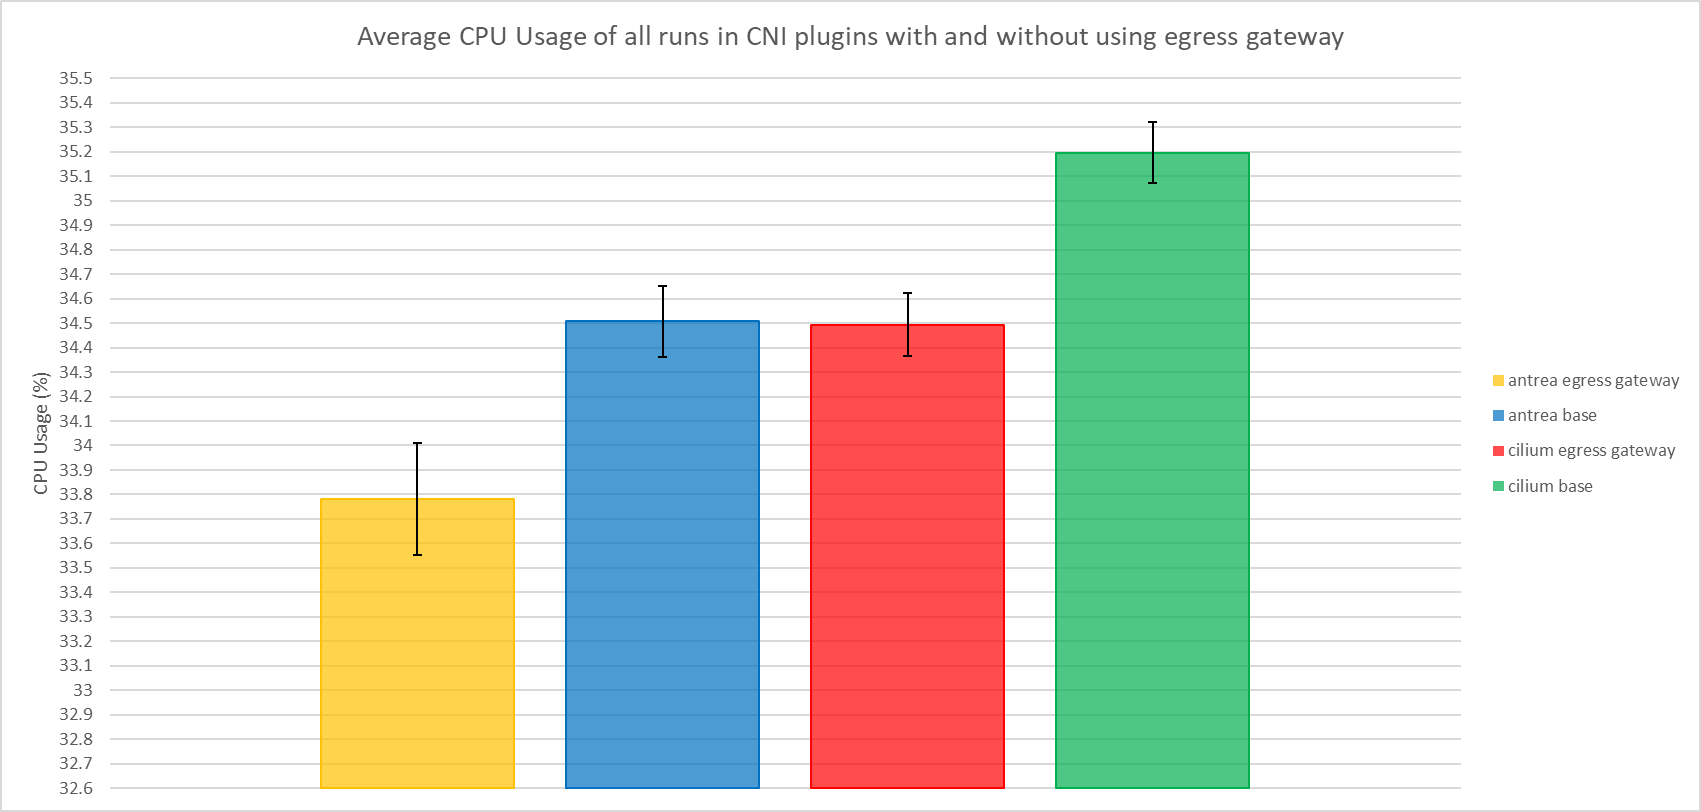
\includegraphics[width=\textwidth]{plots/egress/cpu_total_average.png}
        \caption{}
        \label{fig:cpu_avg}
    \end{subfigure}
    \begin{subfigure}[b]{1\textwidth}
        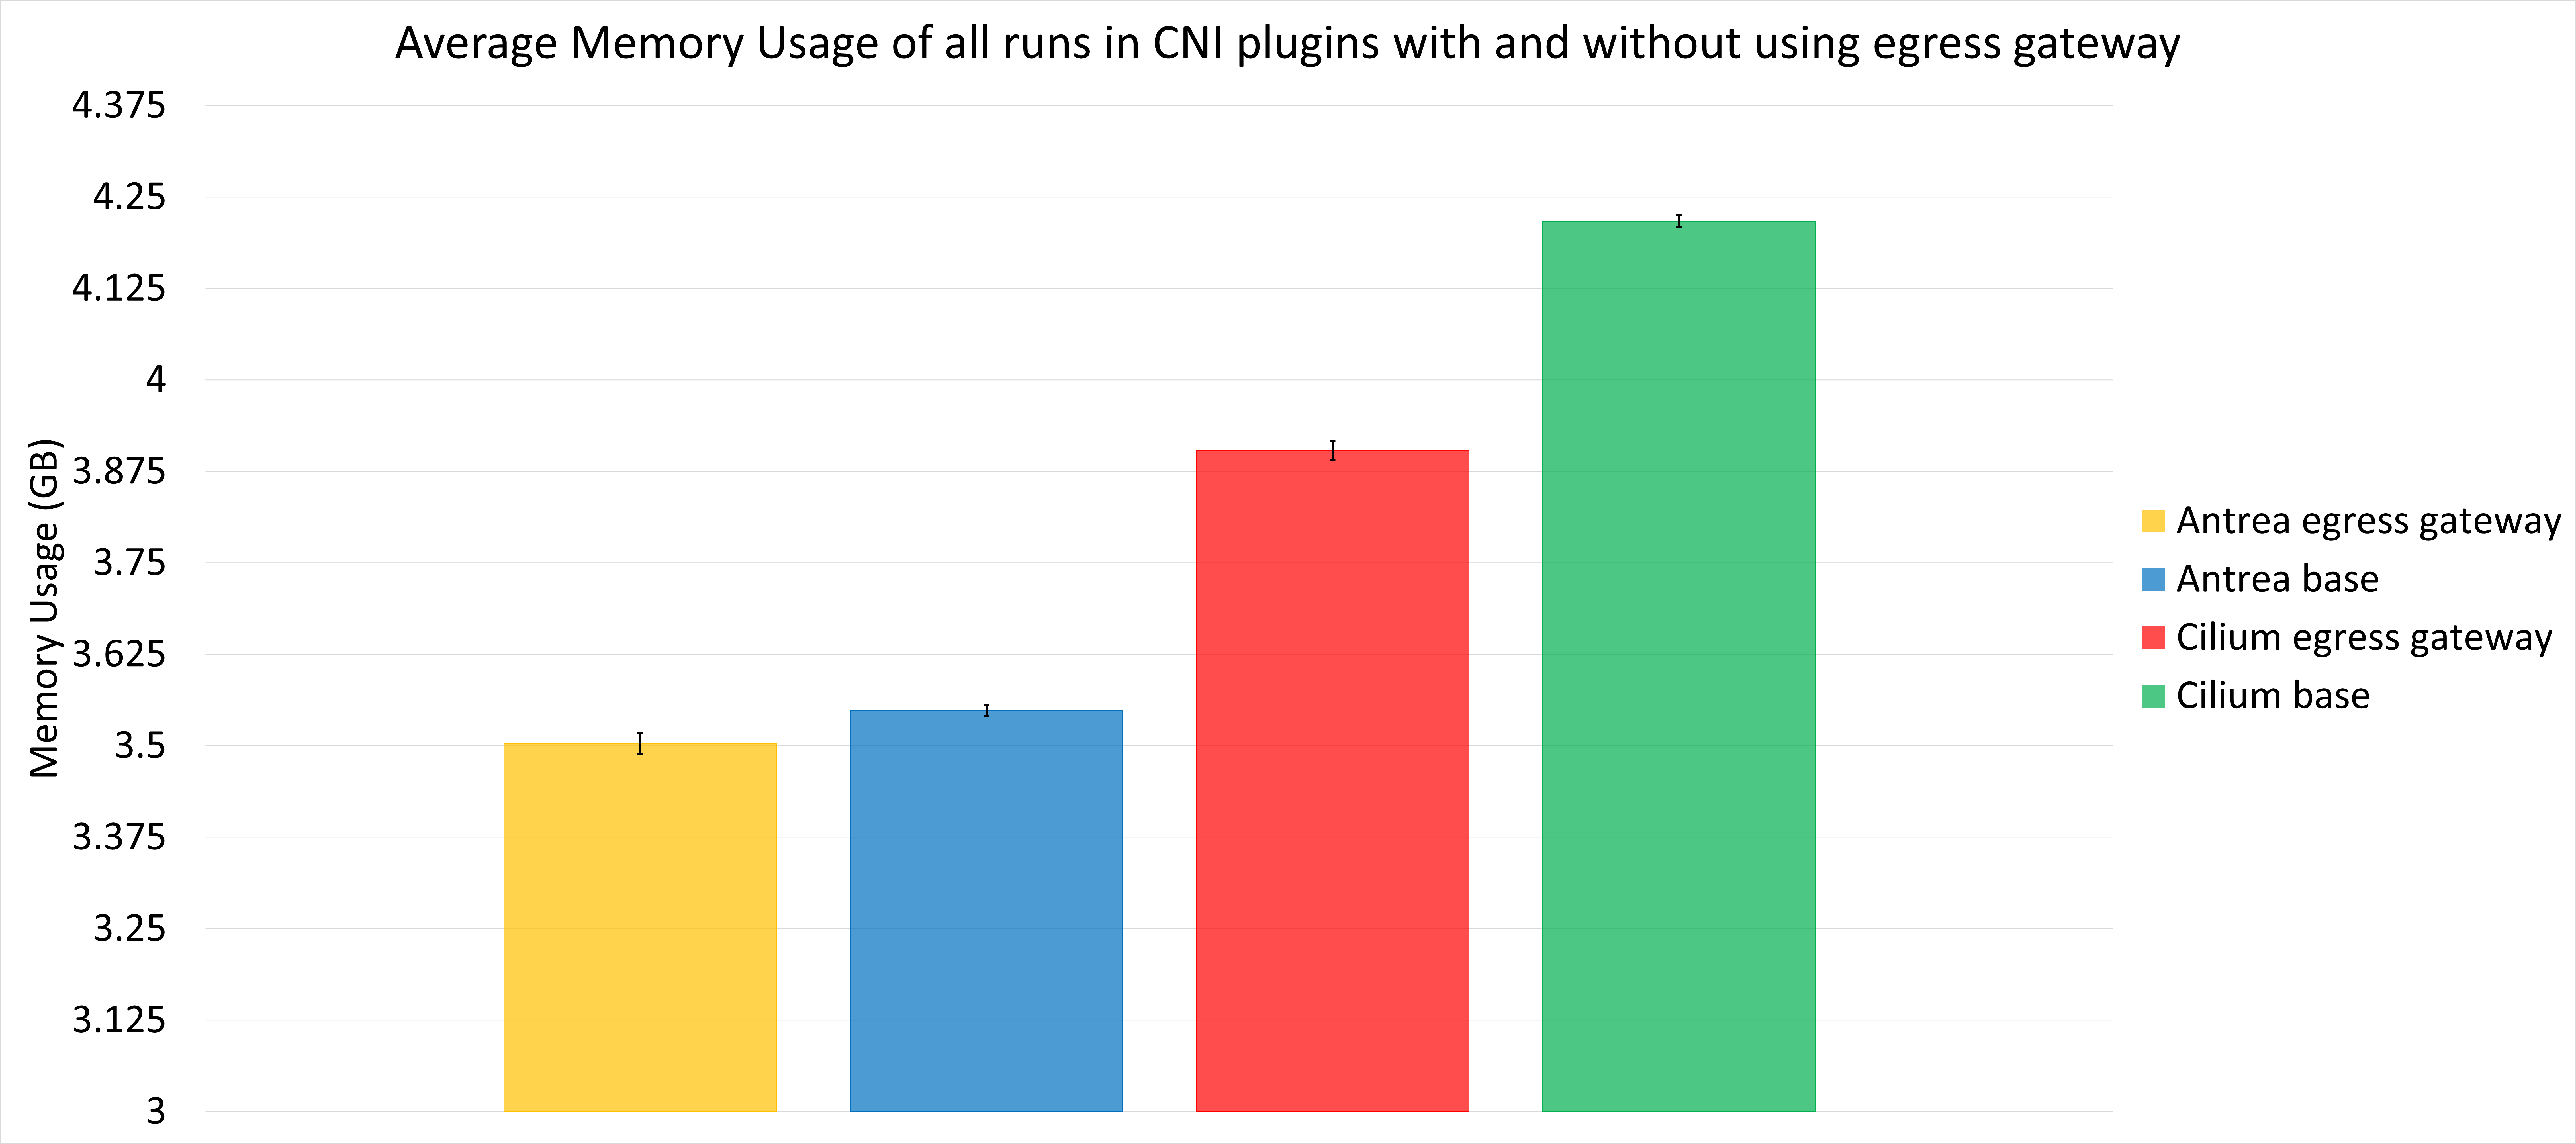
\includegraphics[width=\textwidth]{plots/egress/memory_total_average.png}
        \caption{}
        \label{fig:memory_avg}
    \end{subfigure}
    
    \caption{Average resource consumption in egress scenario, (a) CPU, (b) Memory}
    \label{fig:res_avg}
\end{figure}


\begin{figure}[H]
    \centering
    \begin{subfigure}[b]{1\textwidth}
        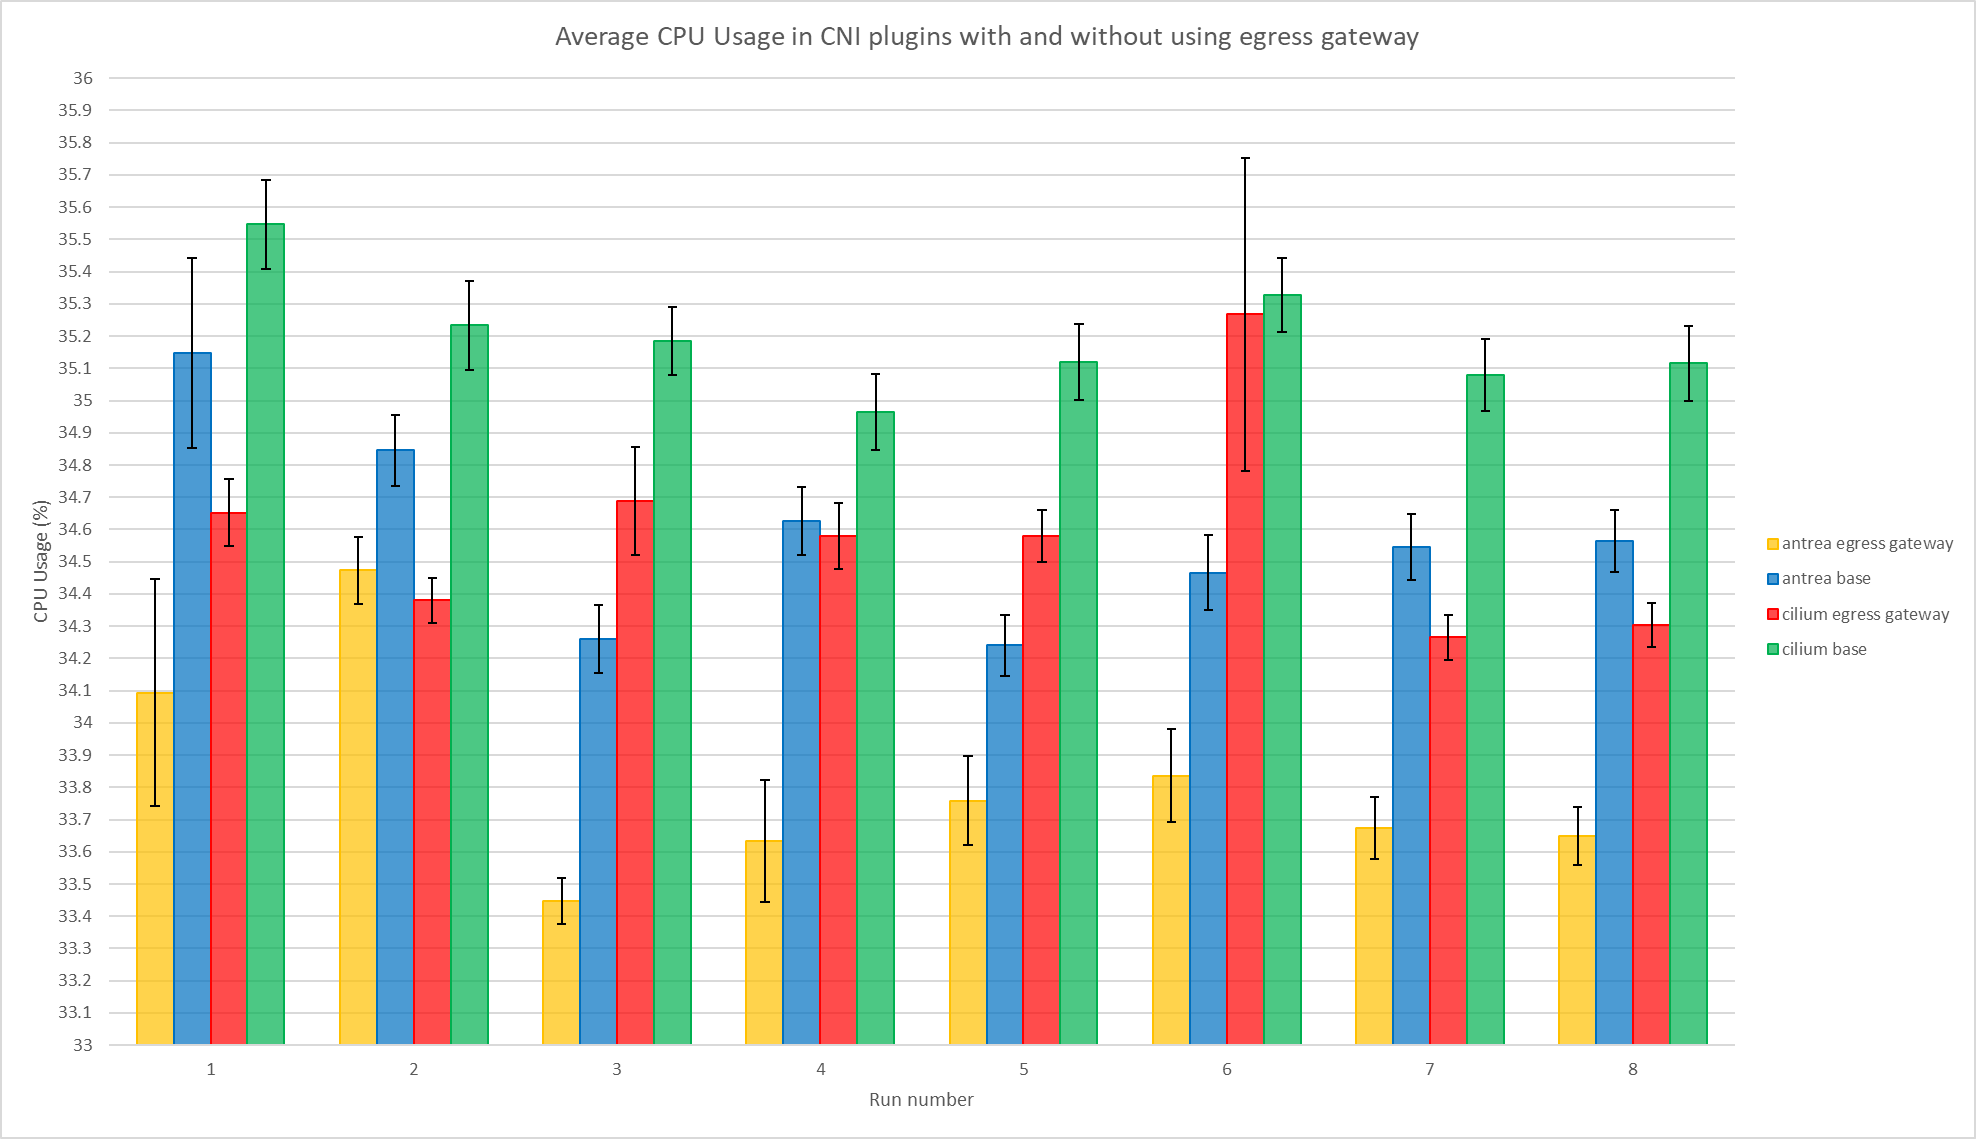
\includegraphics[width=\textwidth]{plots/egress/cpu_all.png}
        \caption{}
        \label{fig:cpu_all}
    \end{subfigure}
    \begin{subfigure}[b]{1\textwidth}
        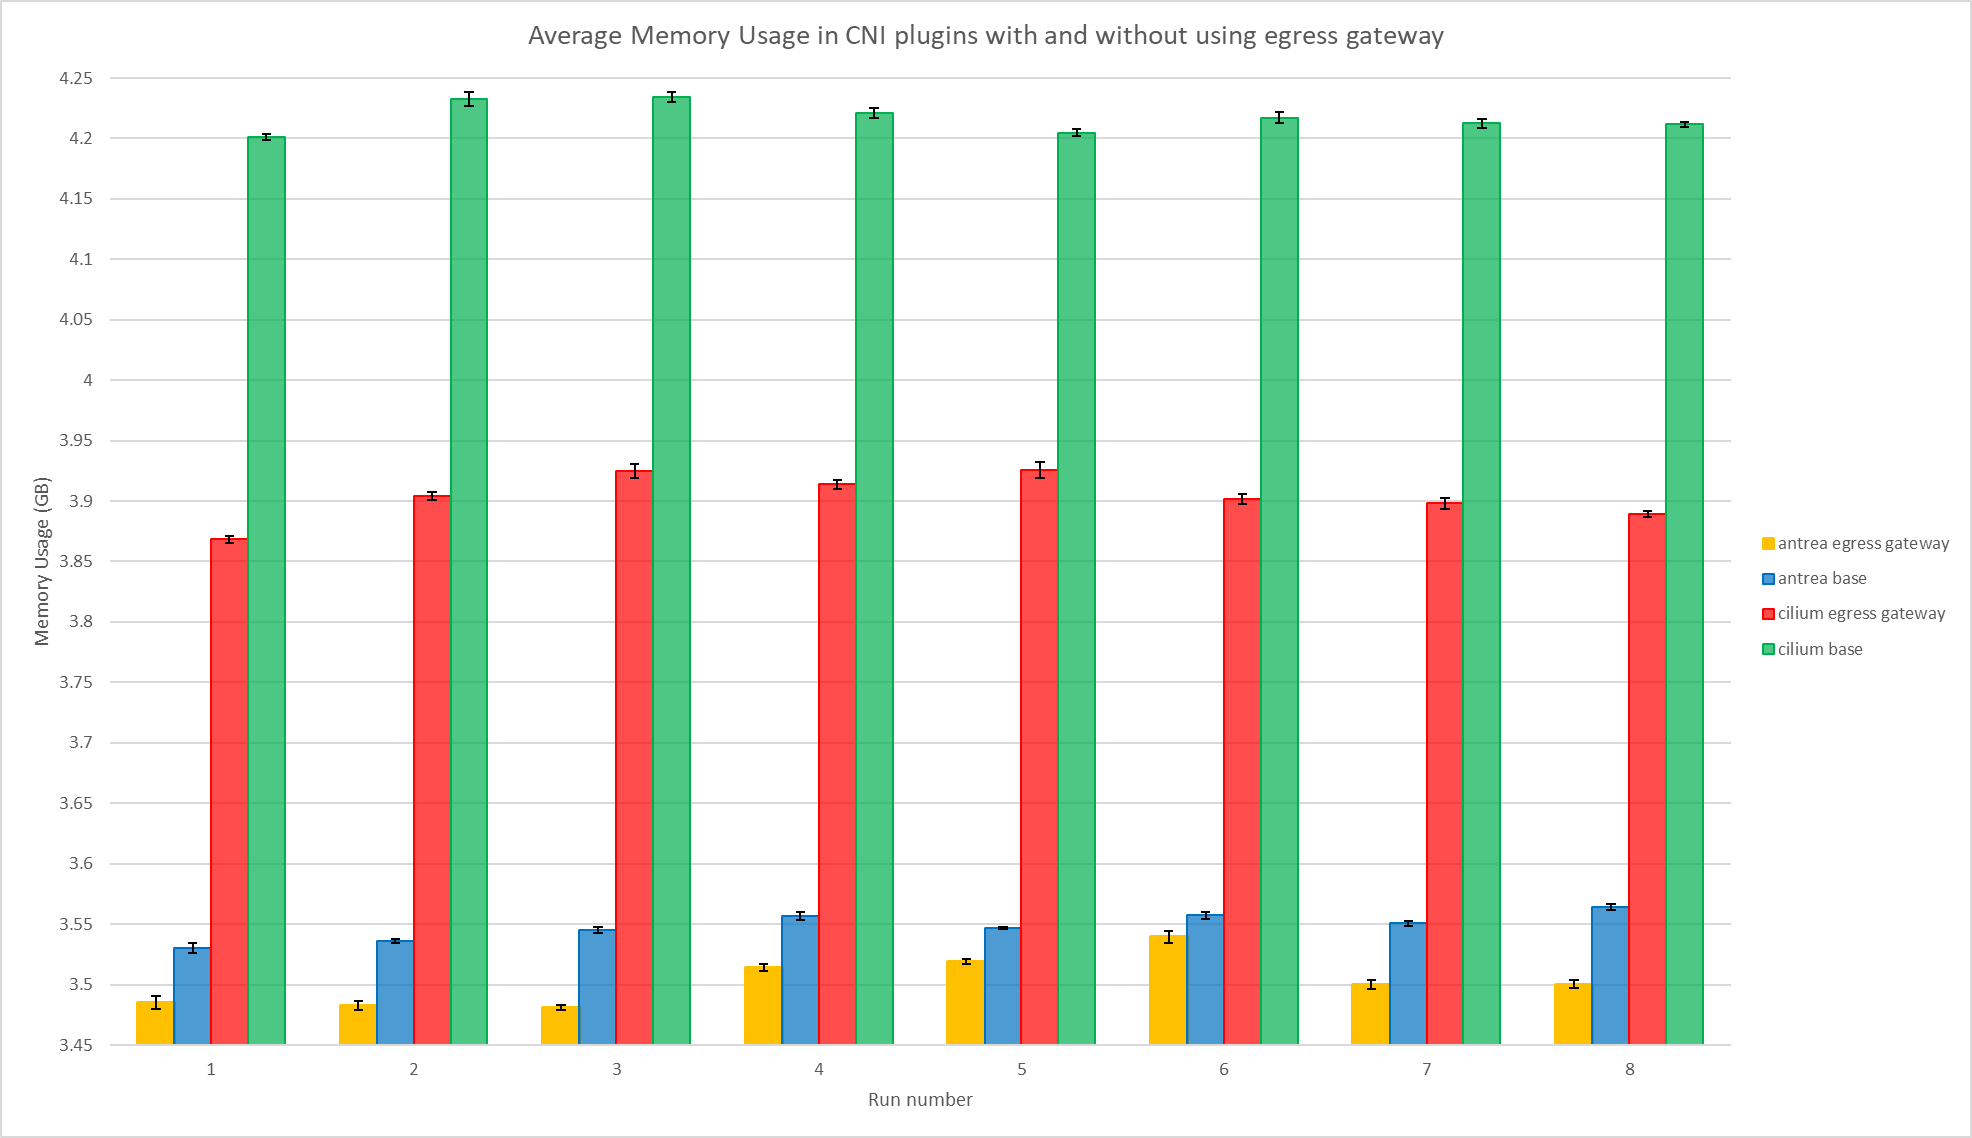
\includegraphics[width=\textwidth]{plots/egress/memory_all.png}
        \caption{}
        \label{fig:memory_all}
    \end{subfigure}
    
    \caption{Average resource consumption in egress scenario in each run, (a) CPU, (b) Memory}
    \label{fig:res_all}
\end{figure}


These figures compare the average CPU and memory usage between Cilium and Antrea CNI across all eight runs. Demonstrates how both container network interface plugins perform under the same test conditions, helping to evaluate which plugin consumes fewer resources. In only the second run did Antrea not use less CPU than Cilium. It also highlights how using an egress gateway with each CNI plugin affects resource usage, compared to scenarios where an egress gateway is not used.



\subsubsection{Networking performance}
\label{sec:egressNetworkingPerformance}

Figures~\ref{fig:throughput_avg} and~\ref{fig:rtt_avg} provide an overall performance summary as the average of all runs. Antrea handles traffic more efficiently, with lower round-trip times, regardless of whether an egress gateway is used. The plots in~\ref{fig:throughput_all} and~\ref{fig:rtt_all} display the results of all eight runs for each test case, showing that Antrea outperforms Cilium in every single run, achieving higher throughput and lower bidirectional latency.

\begin{figure}[H]
    \centering
    \begin{subfigure}[b]{1\textwidth}
        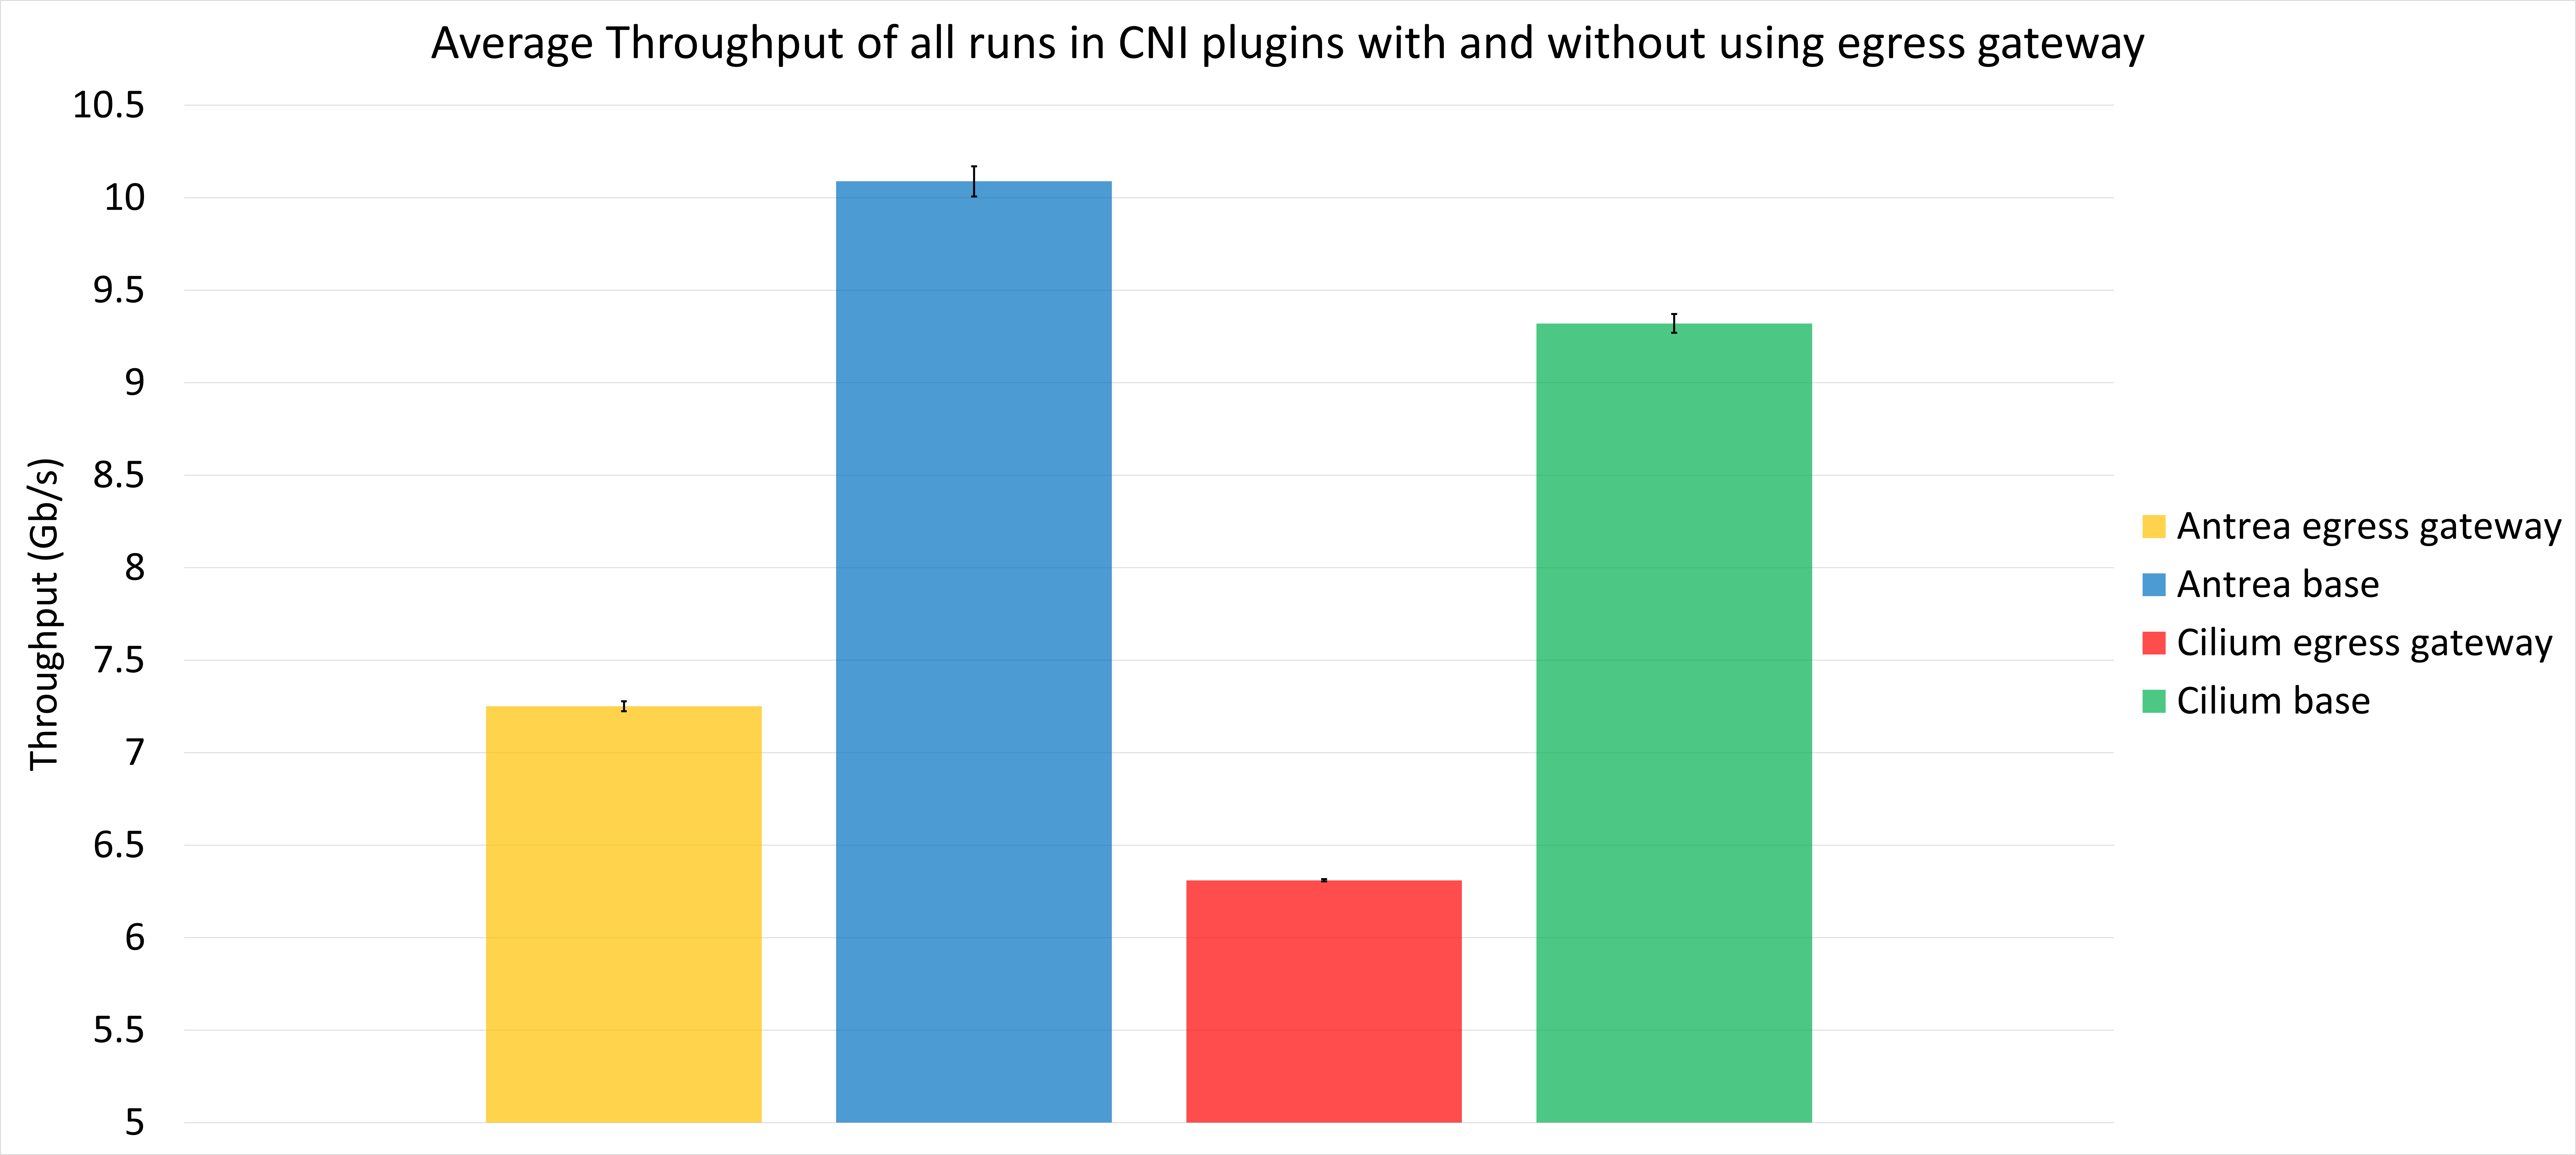
\includegraphics[width=\textwidth]{plots/egress/throughput_total_average.png}
        \caption{}
        \label{fig:throughput_avg}
    \end{subfigure}
    \begin{subfigure}[b]{1\textwidth}
        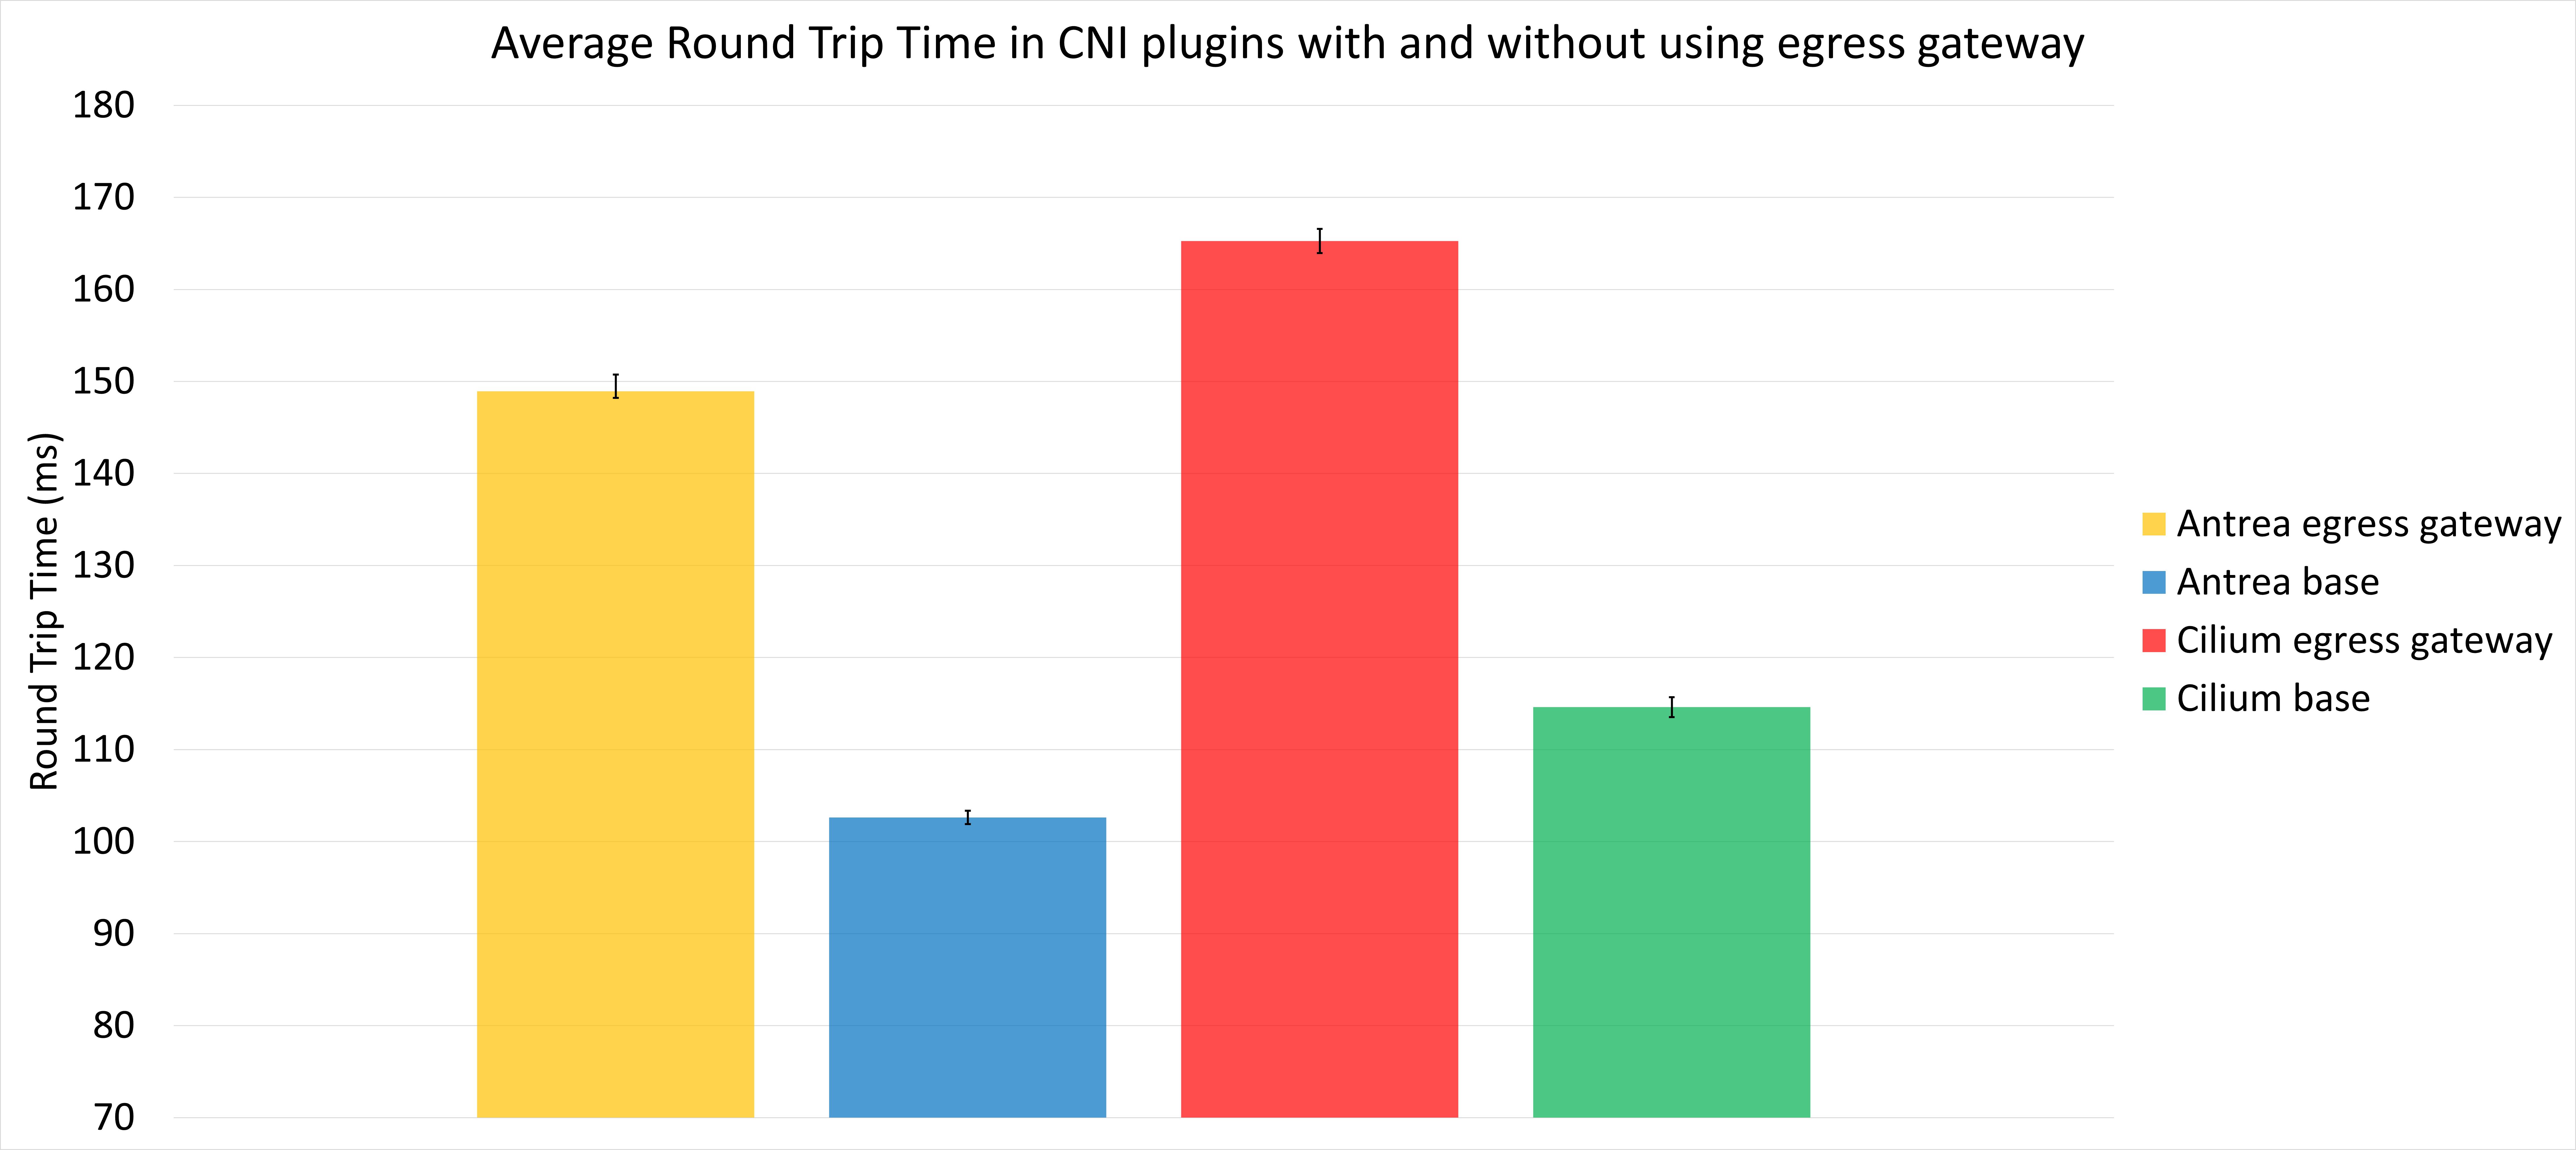
\includegraphics[width=\textwidth]{plots/egress/rtt_total_average.png}
        \caption{}
        \label{fig:rtt_avg}
    \end{subfigure}
    
    \caption{Average networking performance in egress scenario, (a) Throughput, (b) Round Trip Time}
    \label{fig:networking_avg}
\end{figure}

\begin{figure}[H]
    \centering
    \begin{subfigure}[b]{1\textwidth}
        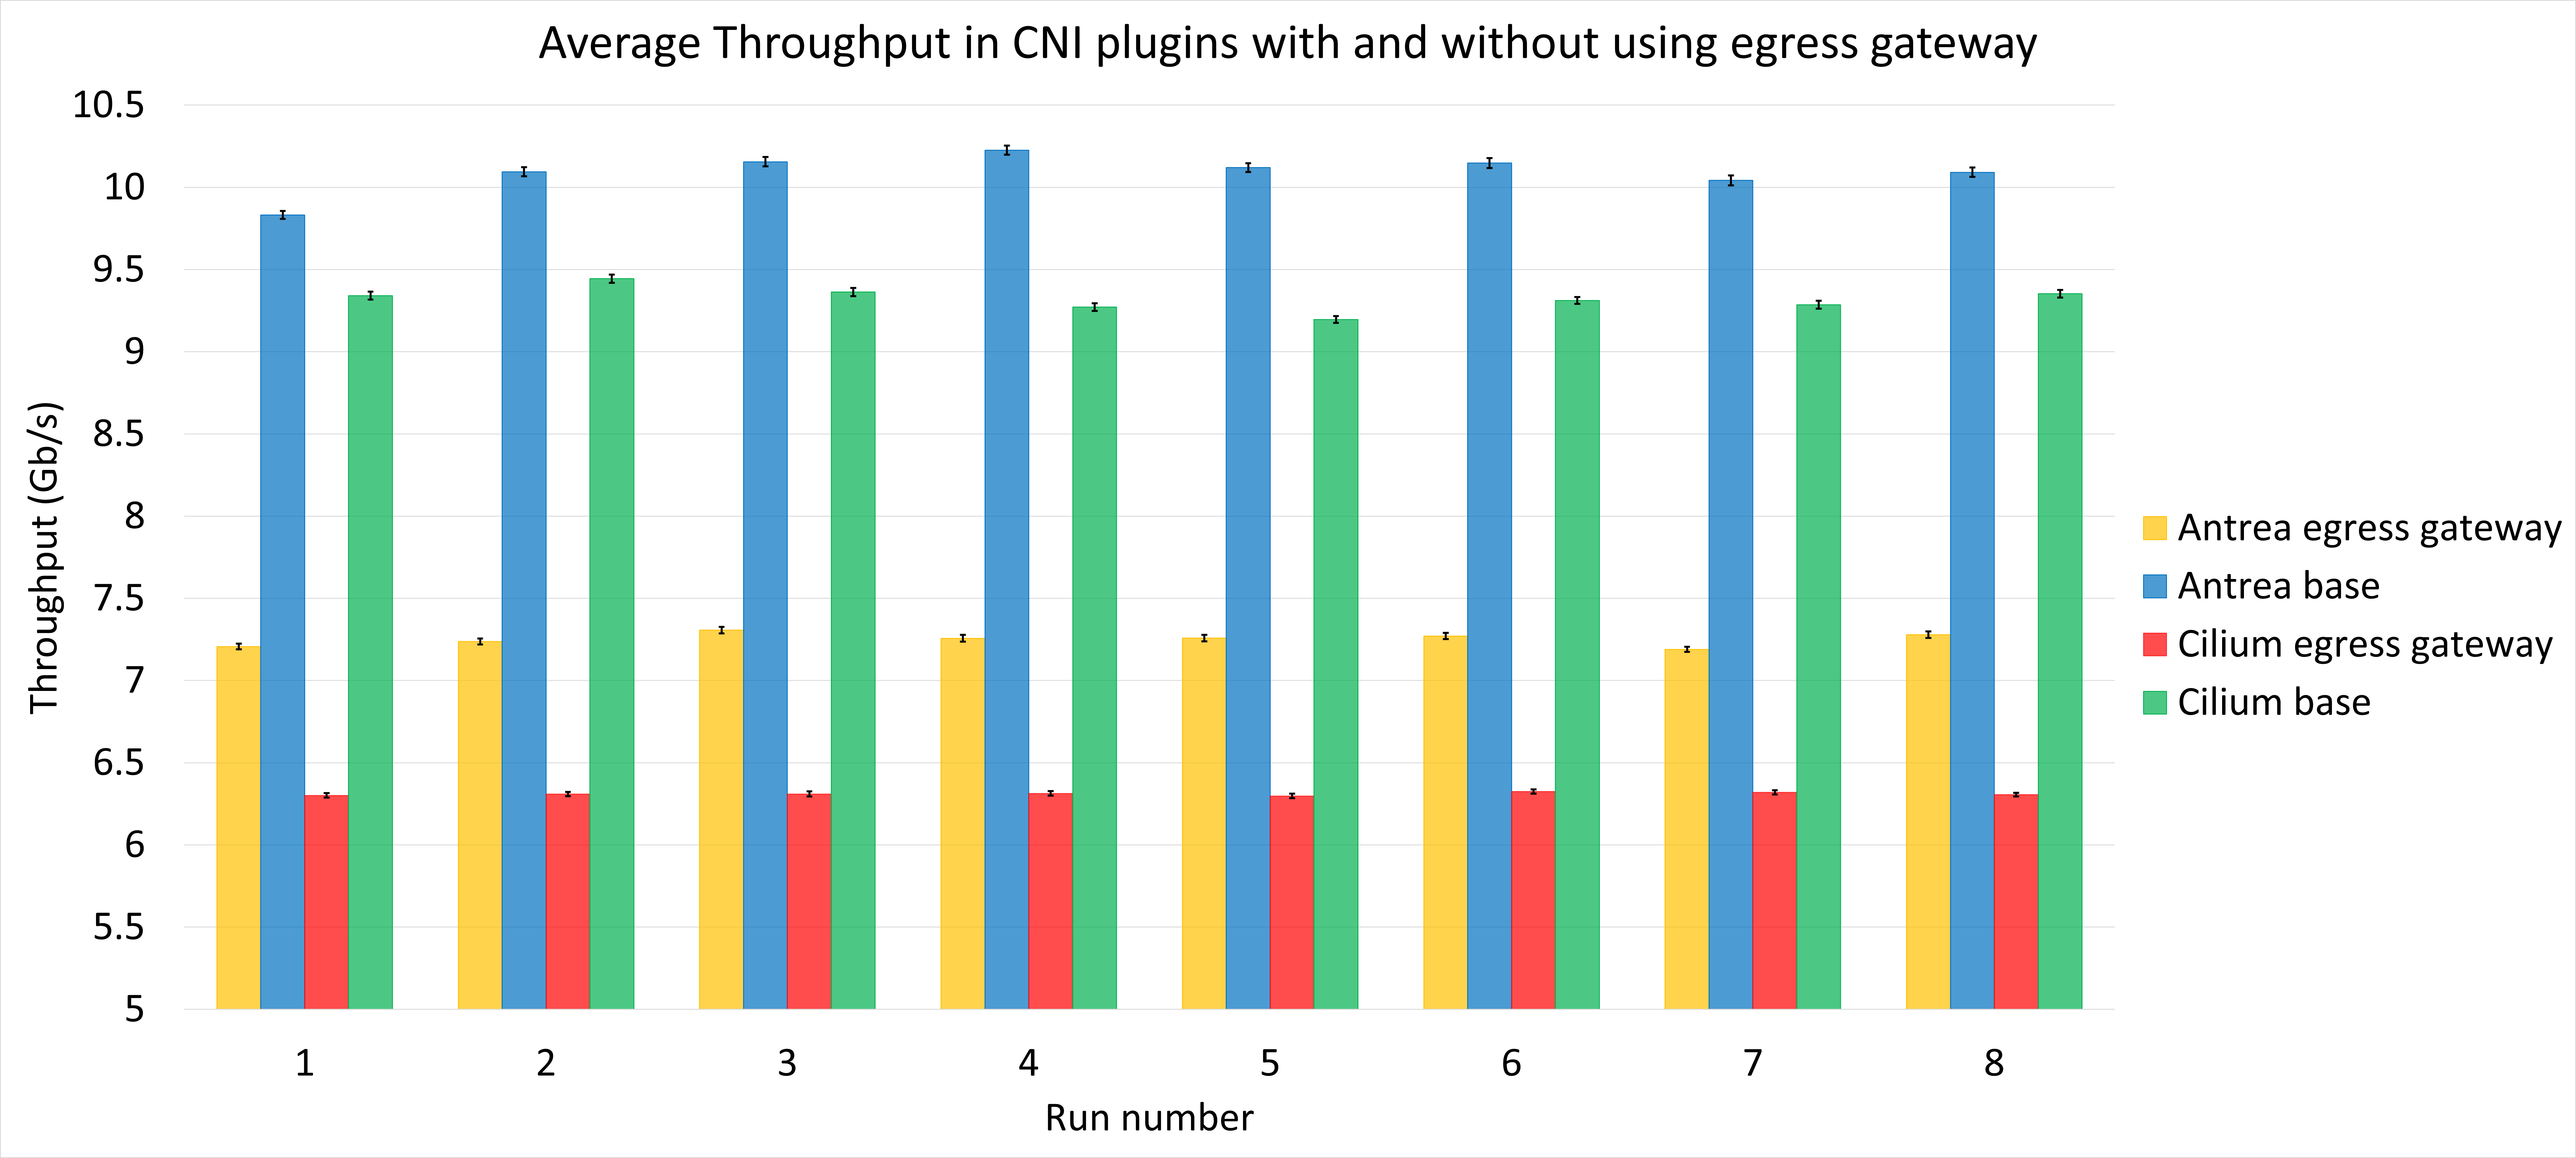
\includegraphics[width=\textwidth]{plots/egress/throughput_all.png}
        \caption{}
        \label{fig:throughput_all}
    \end{subfigure}
    \begin{subfigure}[b]{1\textwidth}
        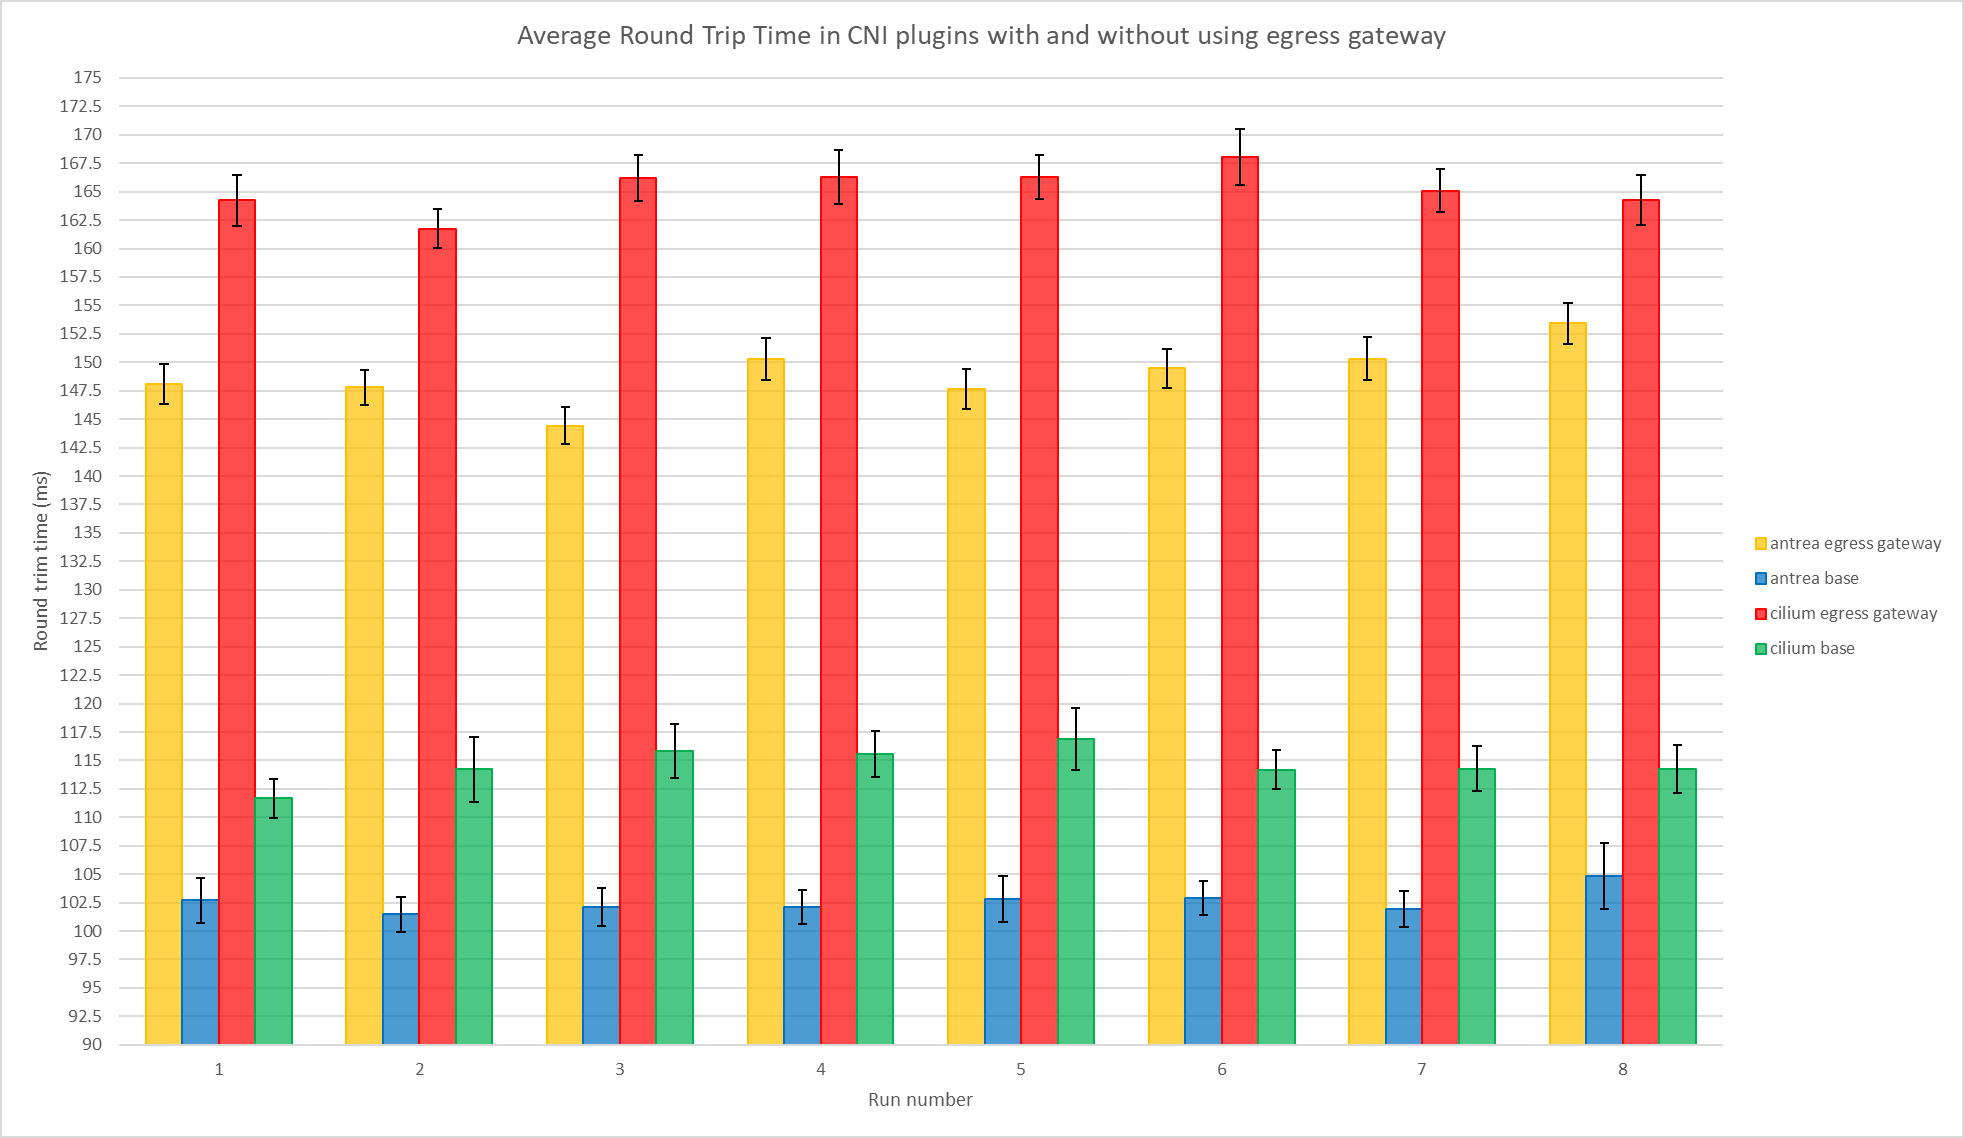
\includegraphics[width=\textwidth]{plots/egress/rtt_all.png}
        \caption{}
        \label{fig:rtt_all}
    \end{subfigure}
    
    \caption{Average networking performance in egress scenario in each run, (a) Throughput, (b) Round Trip Time}
    \label{fig:networking_avg_all}
\end{figure}




Figures~\ref{fig:throughput_all} and~\ref{fig:rtt_all} illustrate the average throughput and round-trip time across eight runs, comparing the performance of the networking plugins. Throughput with the Cilium egress gateway remains stable, hovering around 6.3 Gb/s, with tighter confidence intervals indicating greater stability. In every run, Antrea demonstrates an advantage in both data transfer rate and RTT. It also compare the performance of the CNI plugins with and without the use of an egress gateway. They highlight whether using an egress gateway is beneficial, showing significant differences in throughput and round-trip time.


This performance advantage of Antrea could be attributed to the fact that Cilium uses eBPF, which was designed for large-scale clusters. Since the current cluster consists of only a few pods, eBPF features are not fully leveraged, and Antrea's networking simplicity results in better data rates.

\section{Ingress Scenario}
\label{sec:ingressComparison}

This section presents a comparison of the Antrea and Cilium CNI plugins in ingress scenario. The tests were performed in both local and cloud environments to evaluate their performance.

\subsubsection{Resource consumption}
\label{sec:ingressResoureComsumption}


\begin{figure}[H]
    \centering
    \begin{subfigure}[b]{1\textwidth}
        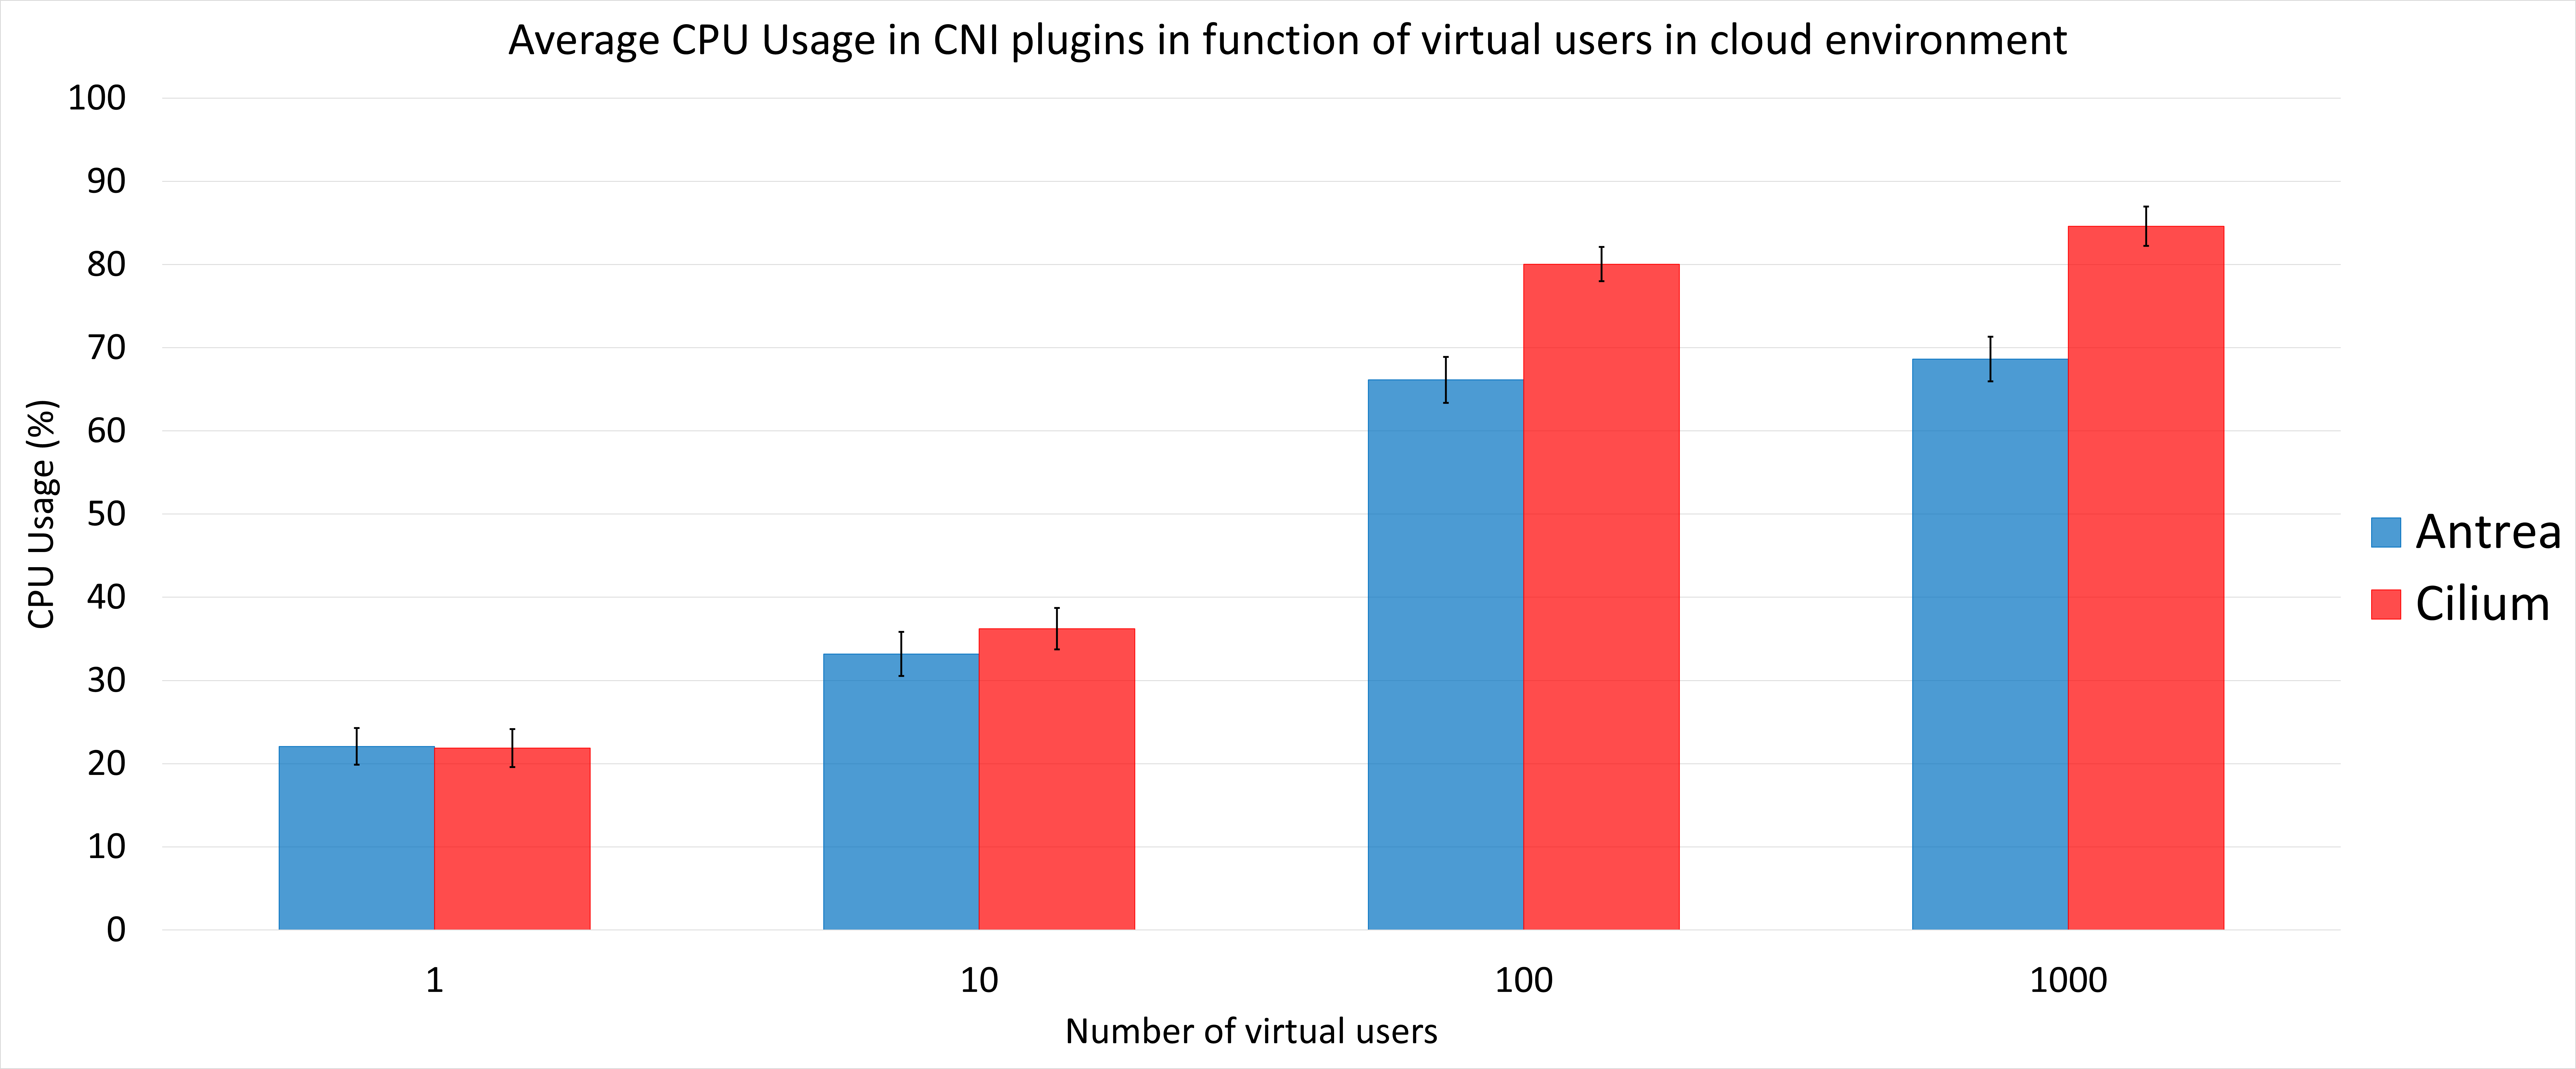
\includegraphics[width=\textwidth]{plots/traffic-splitting/cpu_cloud.png}
        \caption{}
        \label{fig:cpu_cloud_avg}
    \end{subfigure}
    \begin{subfigure}[b]{1\textwidth}
        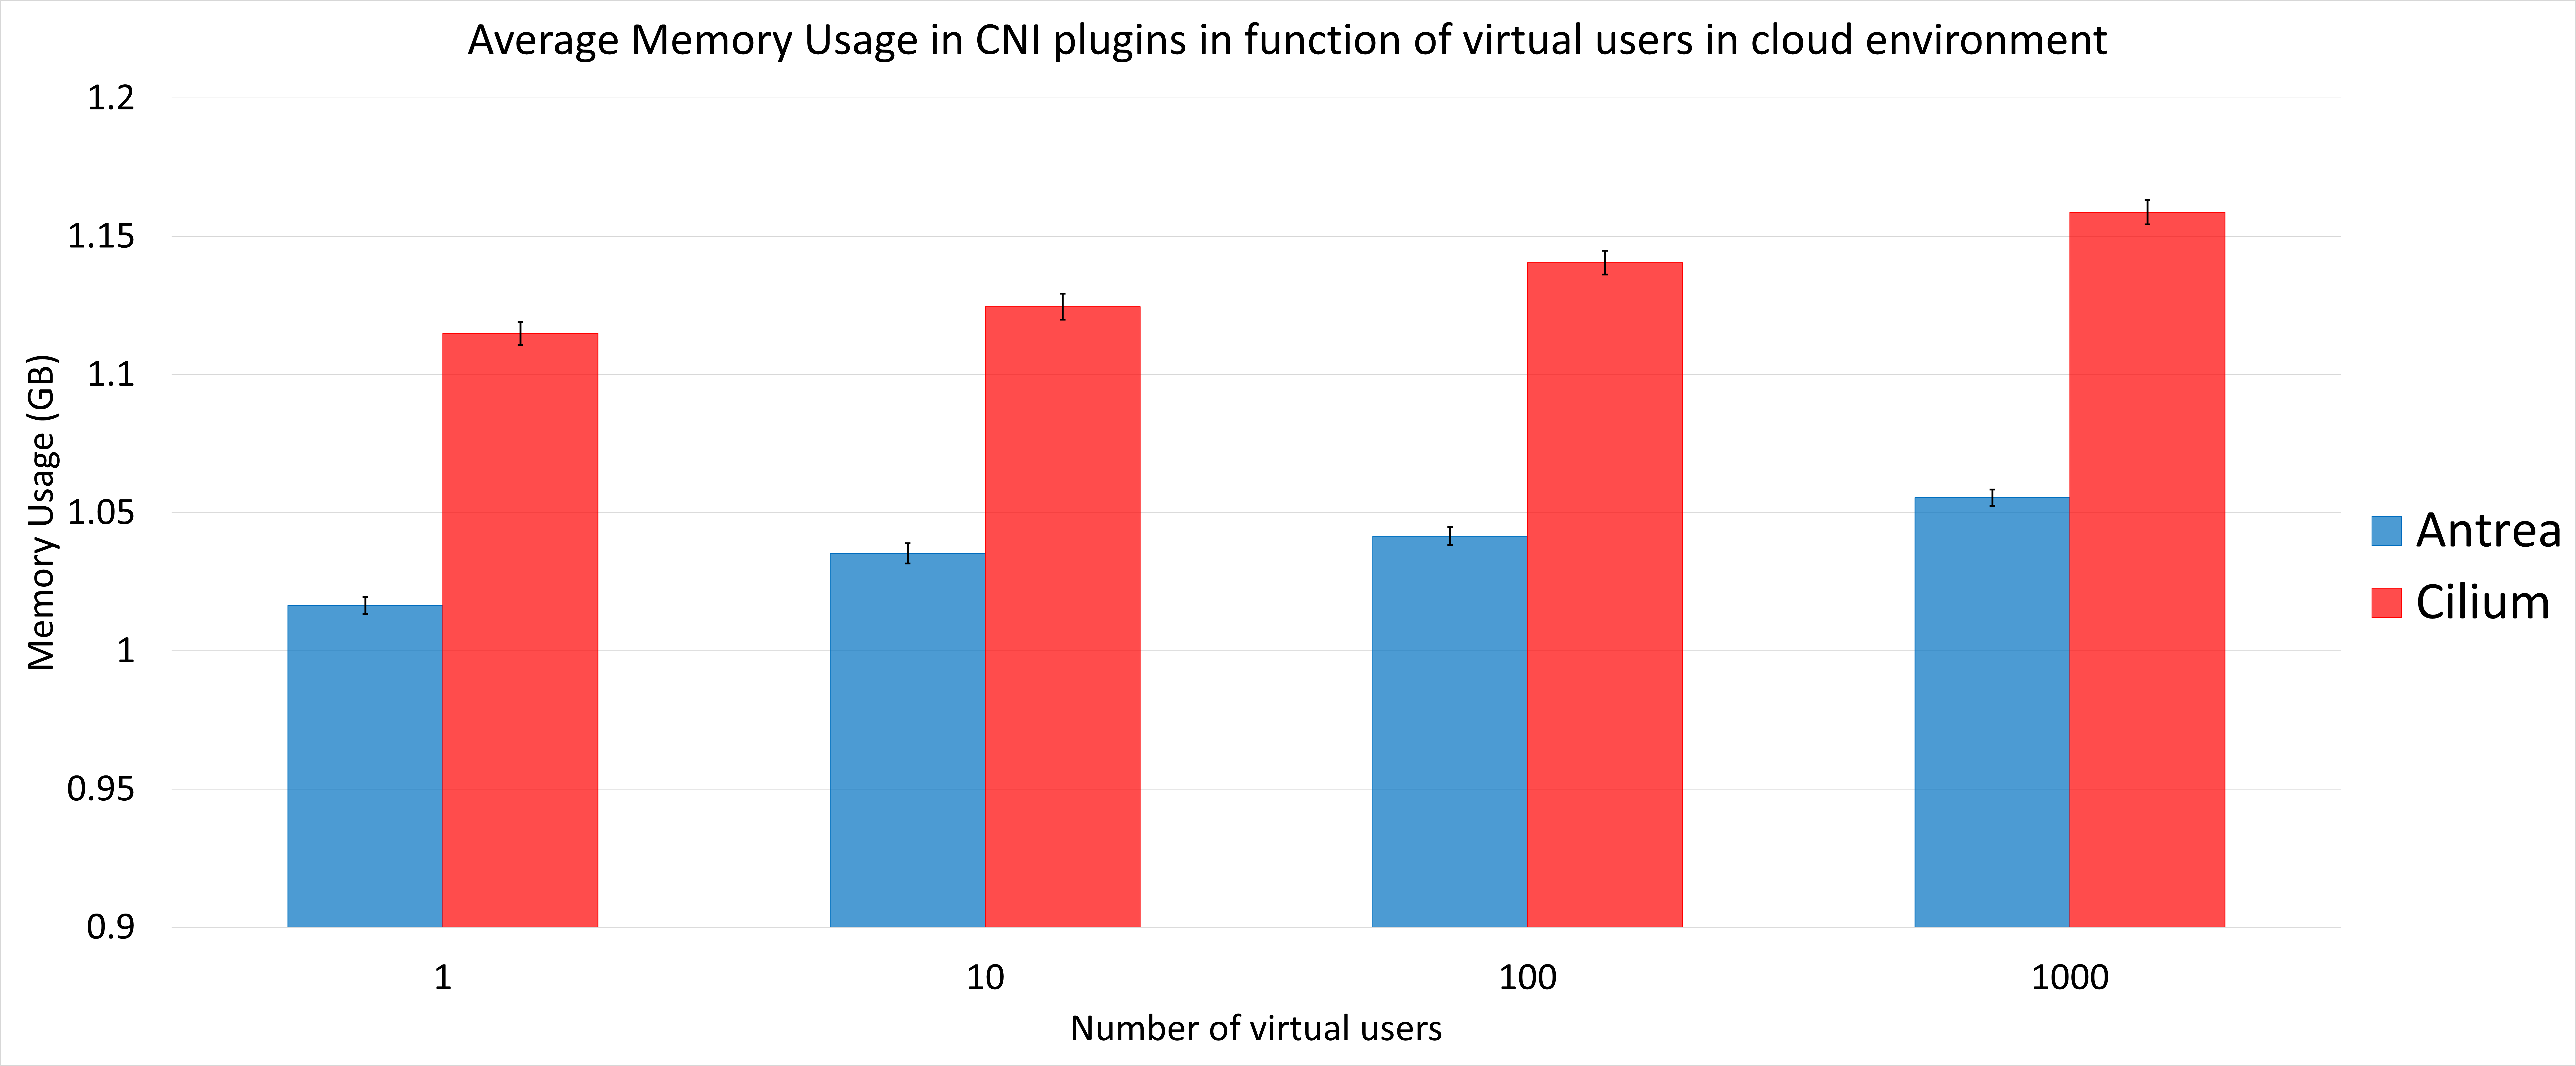
\includegraphics[width=\textwidth]{plots/traffic-splitting/memory_cloud.png}
        \caption{}
        \label{fig:memory_cloud_avg}
    \end{subfigure}
    
    \caption{Average resource utilization in ingress scenario with increasing virtual users in cloud environment, (a) CPU, (b) Memory}
    \label{fig:resource_cloud_avg}
\end{figure}

Comparing Figures~\ref{fig:resource_cloud_avg} and~\ref{fig:resource_local_avg}, it is evident that traffic management primarily impacts CPU usage rather than memory consumption, as memory usage shows egresser increases. In the cloud environment, Antrea demonstrates better resource efficiency, while in the local environment, Cilium consumes fewer resources. Antrea might use more CPU locally because there is an additional node, and the Gateway API NGINX pod is located on a different node (on the control plane) than the pod it forwards data to. This requires more resources to handle traffic across the cluster rather than within a single node.

\begin{figure}[H]
    \centering
    \begin{subfigure}[b]{1\textwidth}
        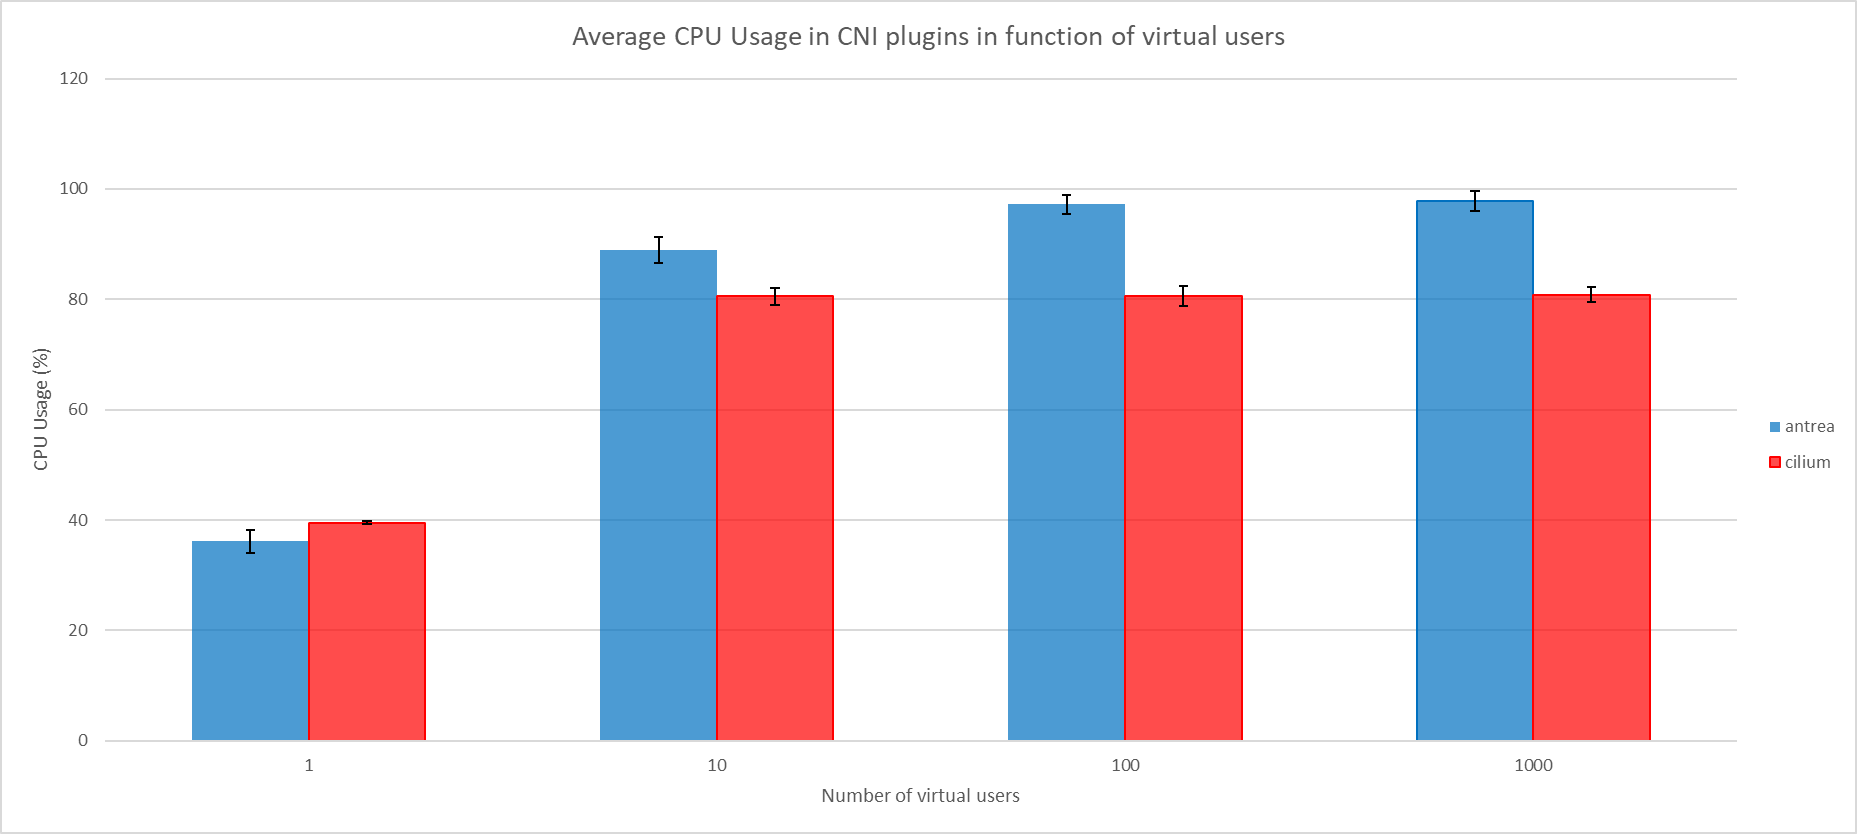
\includegraphics[width=\textwidth]{plots/traffic-splitting/cpu_local.png}
        \caption{}
        \label{fig:cpu_local_avg}
    \end{subfigure}
    \begin{subfigure}[b]{1\textwidth}
        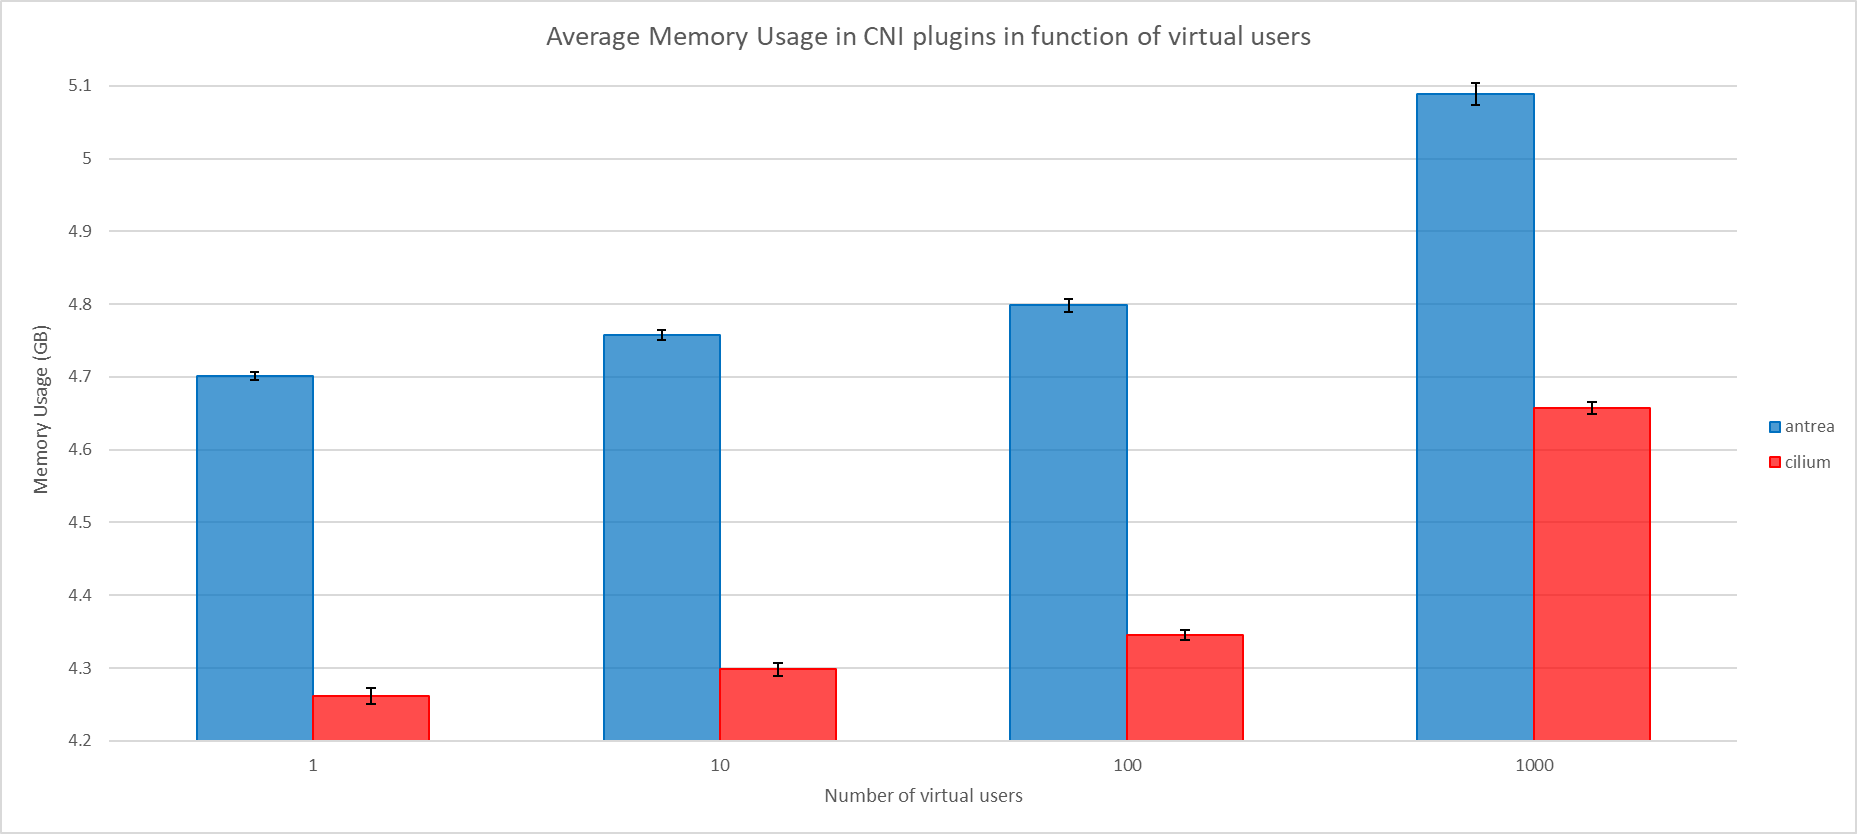
\includegraphics[width=\textwidth]{plots/traffic-splitting/memory_local.png}
        \caption{}
        \label{fig:memory_local_avg}
    \end{subfigure}
    
    \caption{Average resource utilization in ingress scenario with increasing virtual users in local environment, (a) CPU, (b) Memory}
    \label{fig:resource_local_avg}
\end{figure}

\subsubsection{Traffic splitting}
\label{sec:ingressTrafficSplitting}

When comparing traffic weighting accuracy in Figure~\ref{fig:vus_avg} with an increasing number of virtual users in a cloud environment, Antrea proves to be more precise, both when a single user makes a request and when a thousand users generate massive load. In a local environment, Cilium is more accurate in splitting traffic to the value specified in the HTTPRoute in every scenario except when only a single user is involved. Antrea, in the local environment, shows wider confidence intervals, and the distance from the reference point is higher compared to Cilium, making it less effective during high-load periods.


\begin{figure}[H]
    \centering
    \begin{subfigure}[b]{1\textwidth}
        
\includegraphics[width=\textwidth]{plots/traffic-splitting/vus_cloud_all.png}
        \caption{}
        \label{fig:vus_cloud_avg}
    \end{subfigure}
    \begin{subfigure}[b]{1\textwidth}
        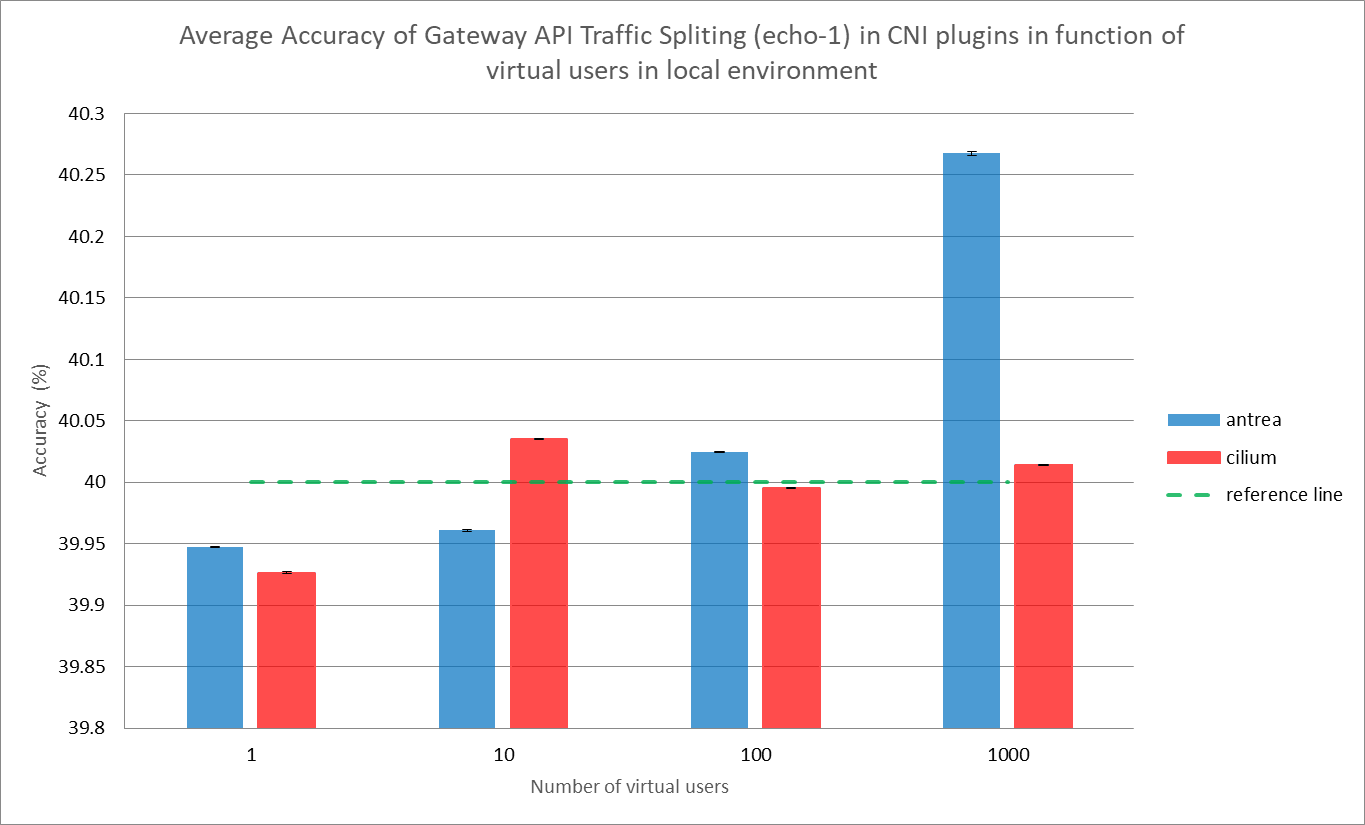
\includegraphics[width=\textwidth]{plots/traffic-splitting/vus_local_all.png}
        \caption{}
        \label{fig:vus_local_avg}
    \end{subfigure}
    
    \caption{Average traffic splitting accuracy in ingress scenario with increasing virtual users (a) cloud, (b) local}
    \label{fig:vus_avg}
\end{figure}


Analyzing the plots in Figure~\ref{fig:avg_vus}, we observe overlapping confidence intervals in all cases, indicating some variability in the results. However, when averaging the values, it becomes clear that Cilium performs better, particularly when the number of virtual users (VUs) is either one or a thousand. The distance to reference points is illustrated in Figure~\ref{fig:referencesIngress}. Although the overlapping confidence intervals suggest statistical uncertainty, the average values show that Cilium achieves higher accuracy in traffic weighting compared to Antrea and the NGINX test case.


\begin{figure}[H]
    \centering
    \begin{subfigure}[b]{0.85\textwidth}
        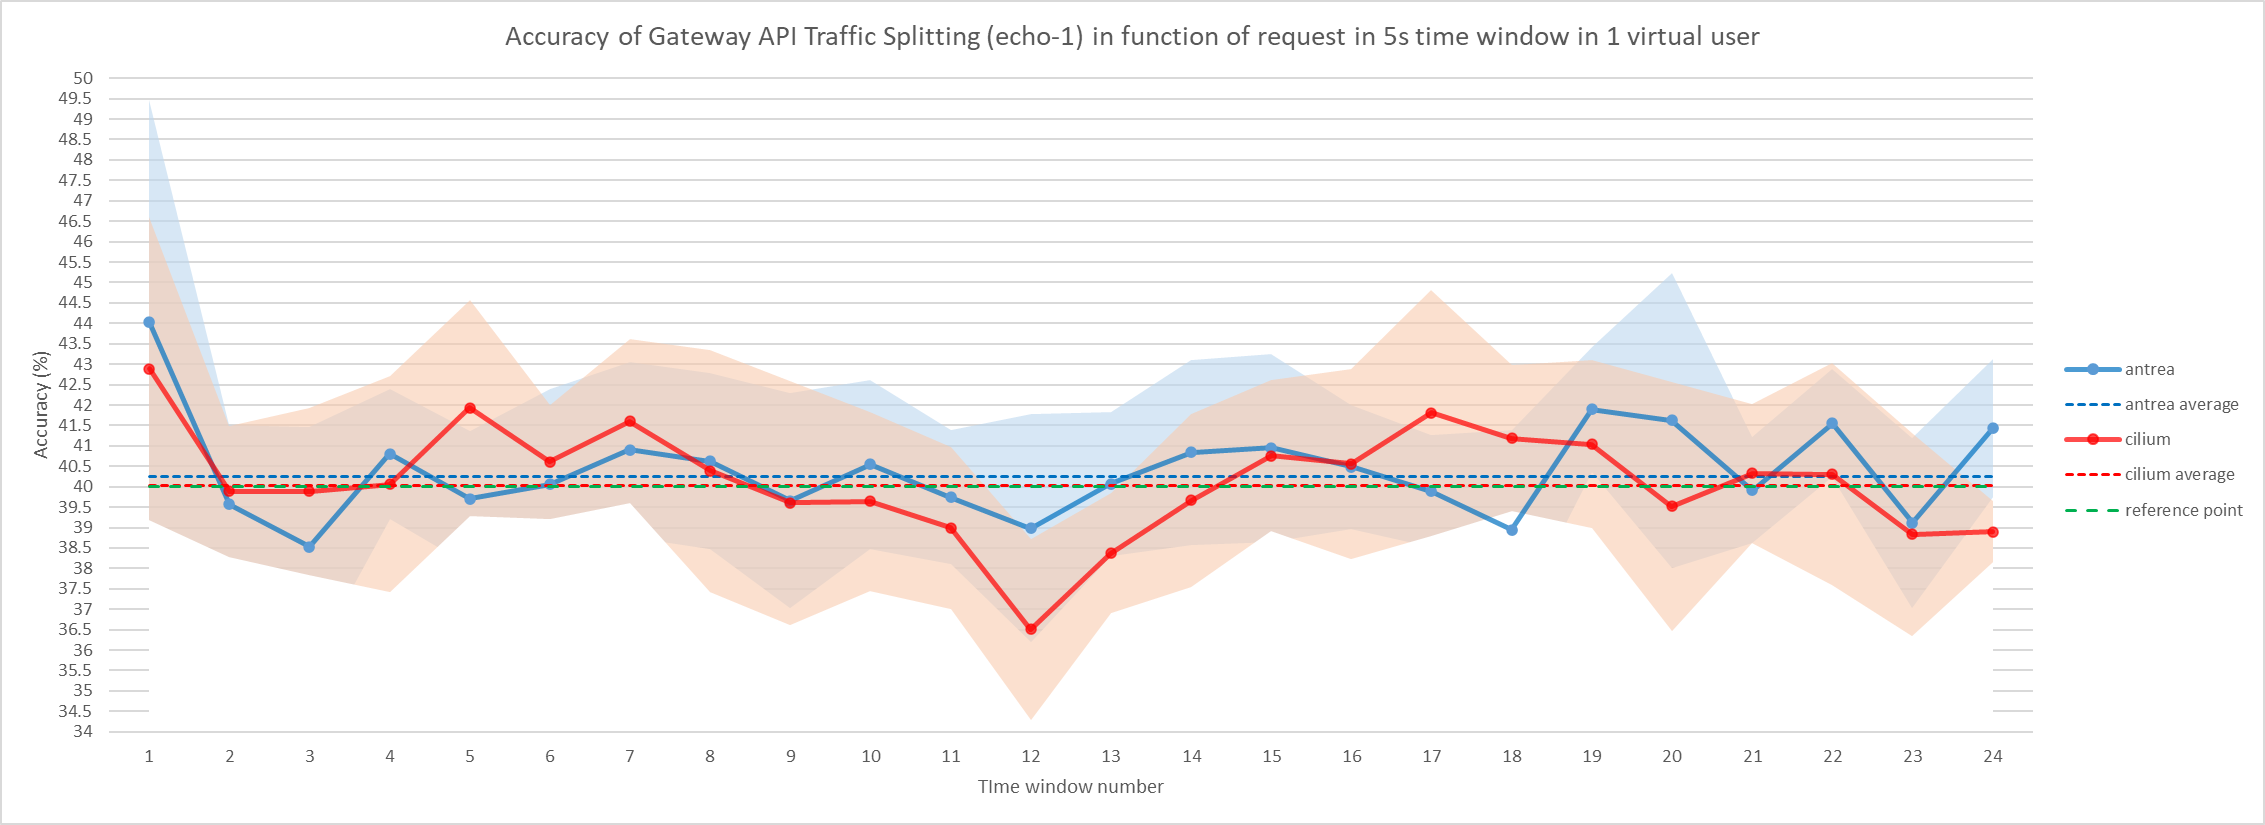
\includegraphics[width=\textwidth]{plots/traffic-splitting/time_window_5_1vu_cloud.png}
        \label{fig:time_window_1vu}
    \end{subfigure}

    \vspace{-0.5cm}

    \begin{subfigure}[b]{0.85\textwidth}
        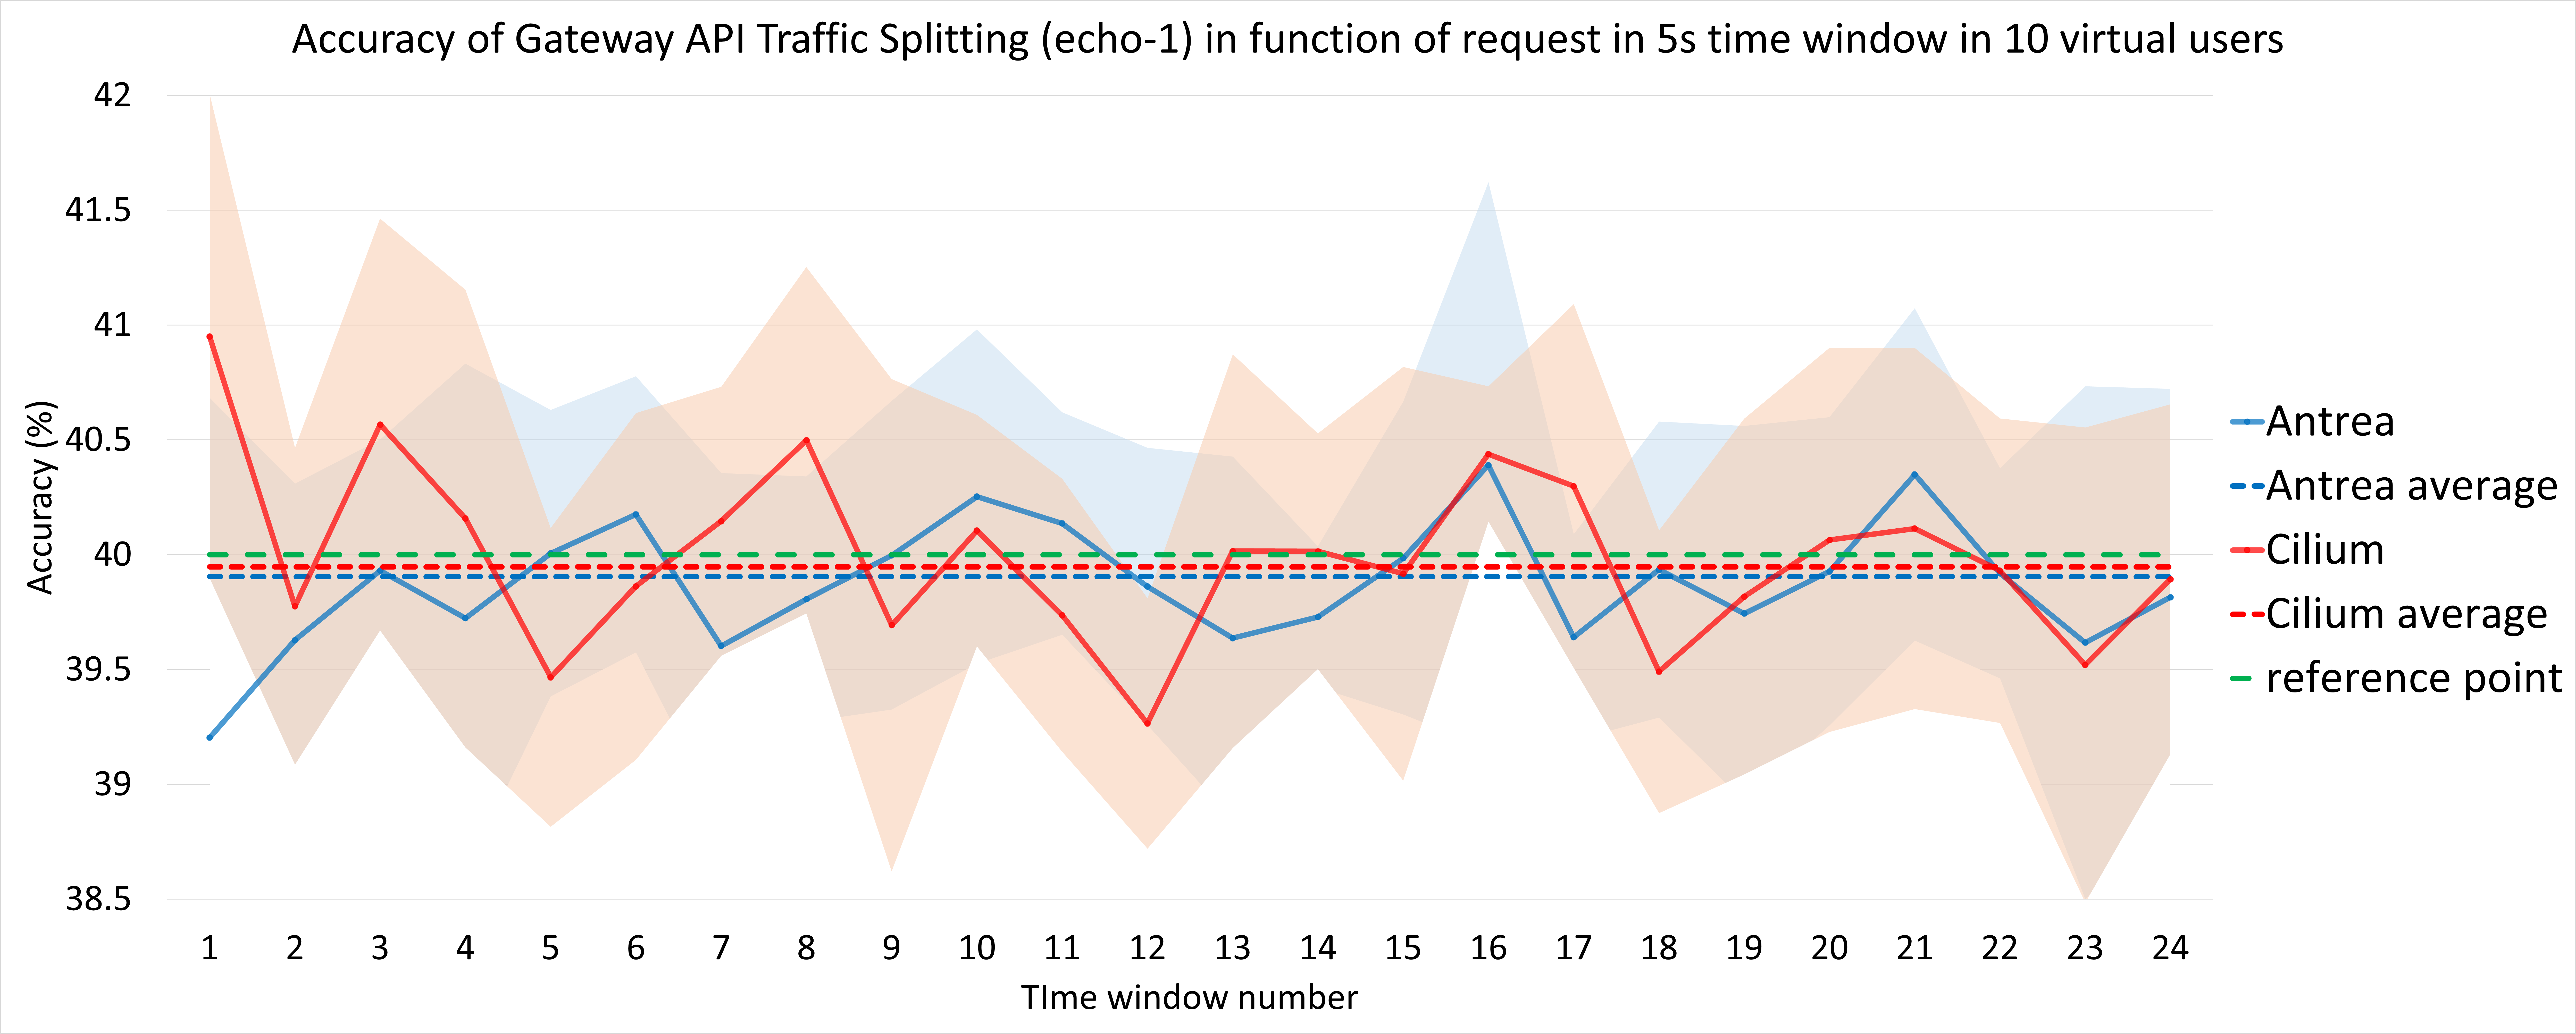
\includegraphics[width=\textwidth]{plots/traffic-splitting/time_window_5_10vu_cloud.png}
        \label{fig:time_window_10vu}
    \end{subfigure}

    \vspace{-0.5cm}

    \begin{subfigure}[b]{0.85\textwidth}
        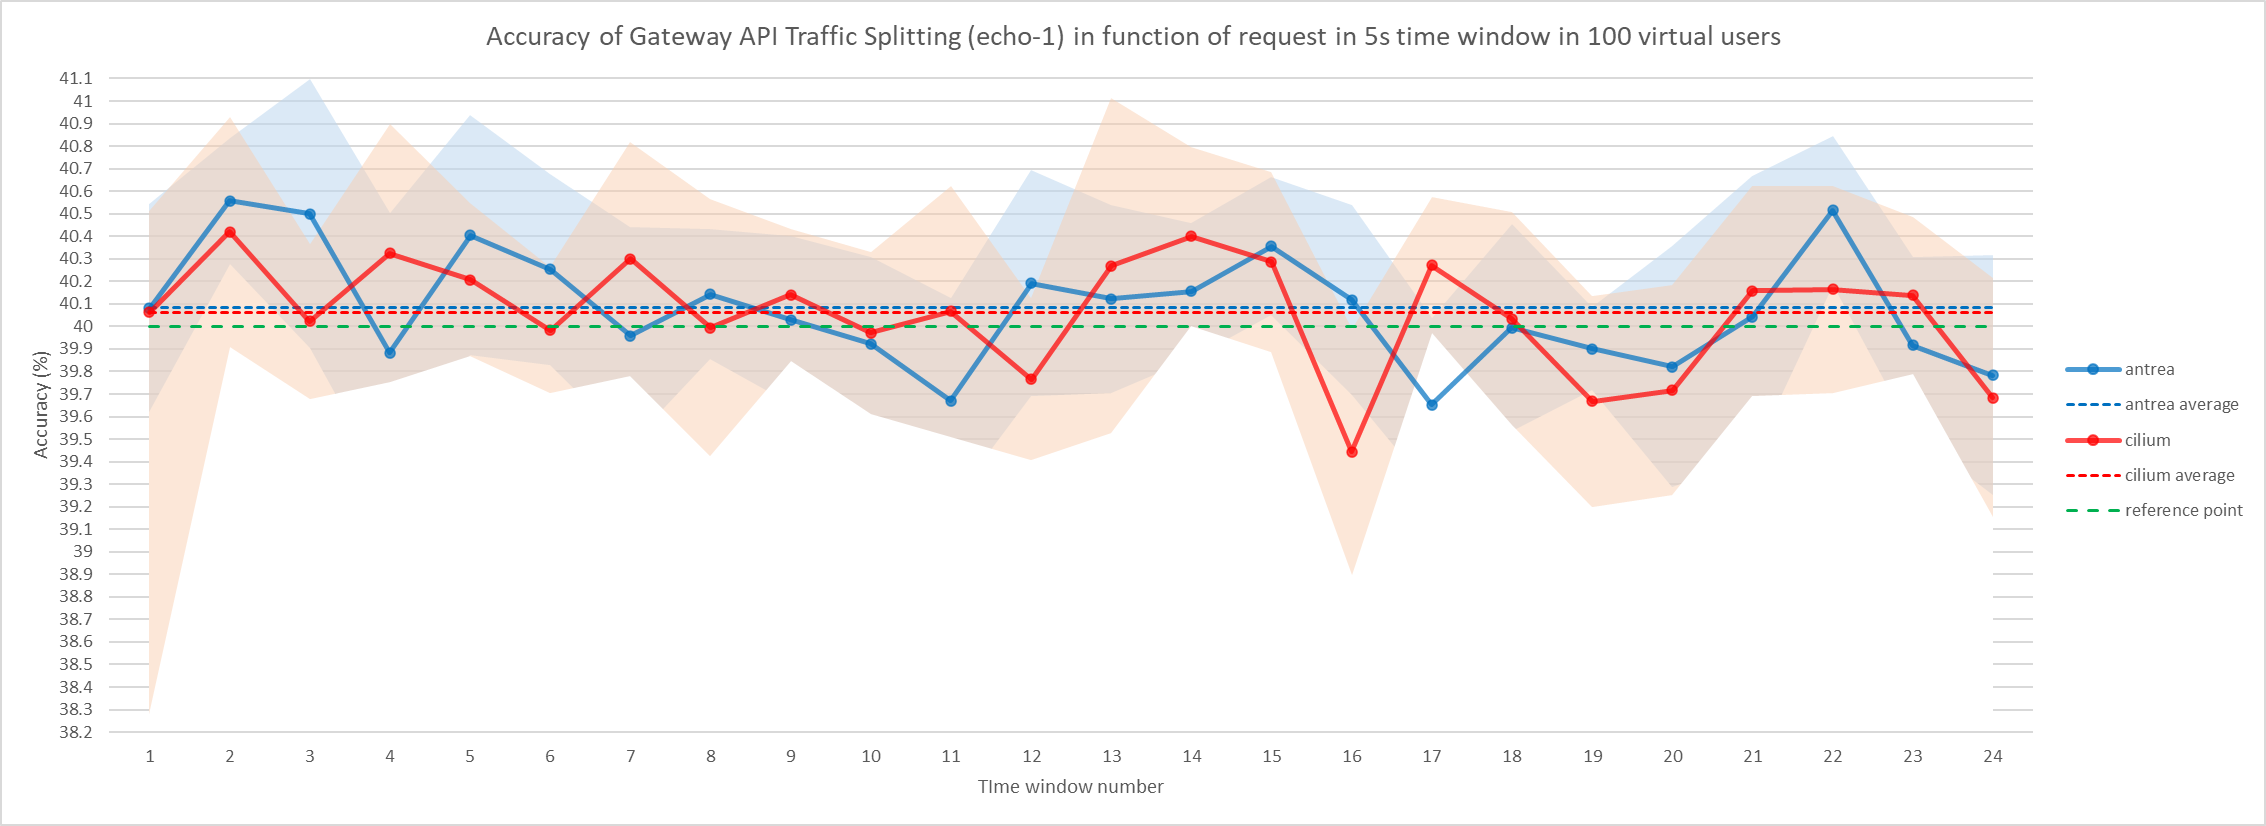
\includegraphics[width=\textwidth]{plots/traffic-splitting/time_window_5_100vu_cloud.png}
        \label{fig:time_window_100vu}
    \end{subfigure}

    \vspace{-0.5cm}

    \begin{subfigure}[b]{0.85\textwidth}
        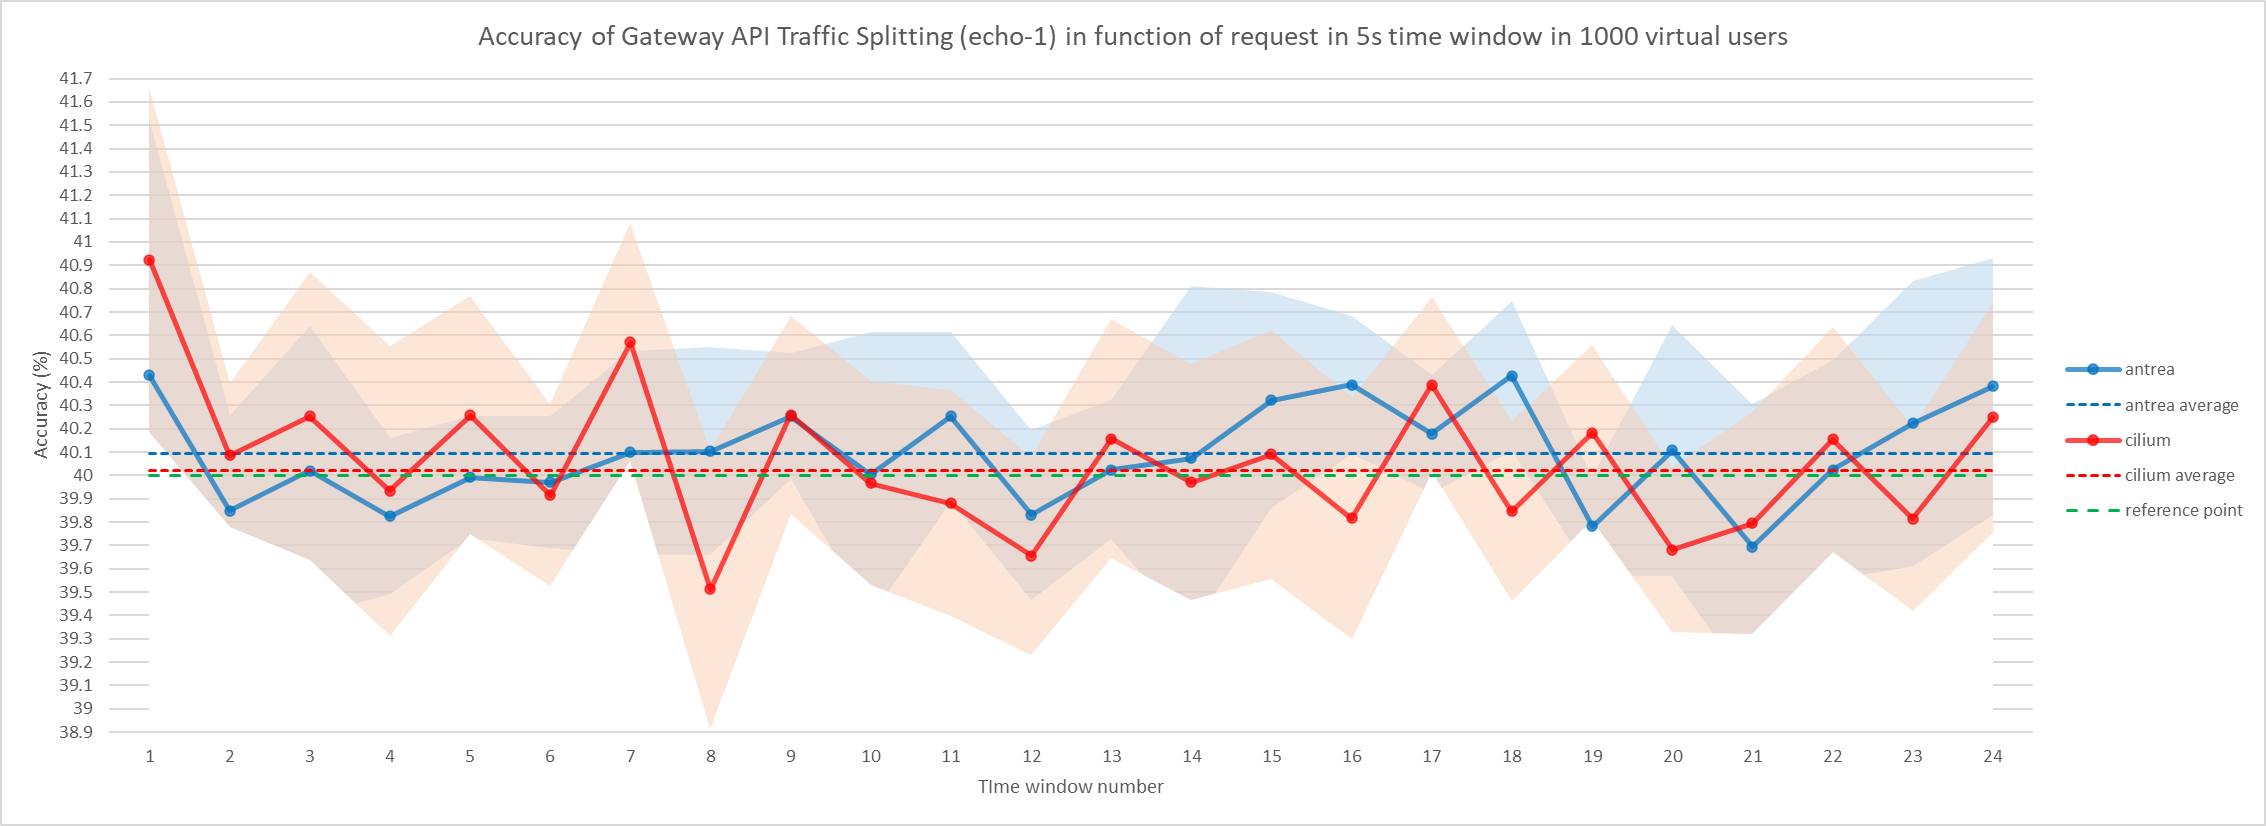
\includegraphics[width=\textwidth]{plots/traffic-splitting/time_window_5_1000vu_cloud.png}
        \label{fig:time_window_1000vu}
    \end{subfigure}

    \vspace{-0.3cm}

    \caption{Average traffic splitting ratio in function of five second request time windows with increasing virtual users; one, ten, a hundred and a thousand users}
    \label{fig:avg_vus}
\end{figure}



\begin{figure}[H]
    \centering
    \begin{subfigure}[b]{0.49\textwidth}
        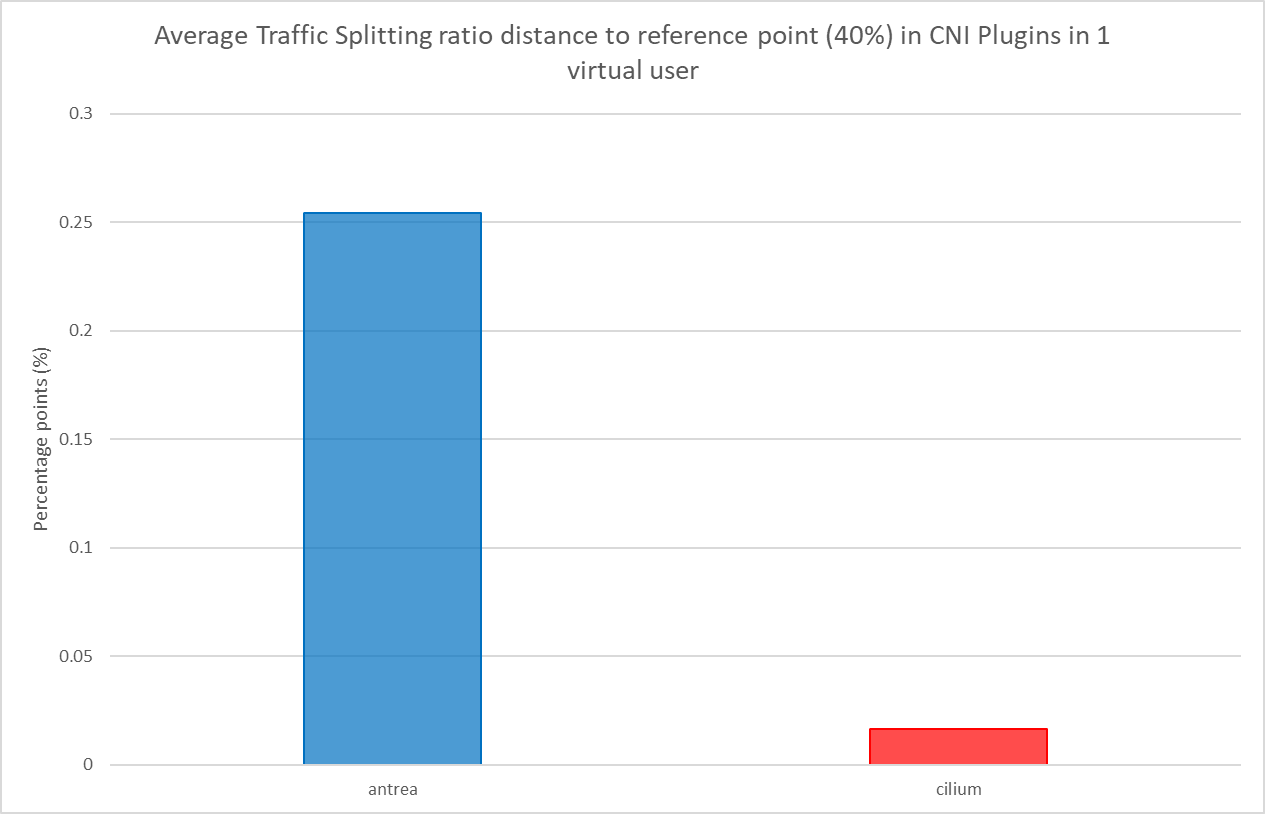
\includegraphics[width=\textwidth]{plots/traffic-splitting/time_window_5_1vu_reference_cloud.png}
        \label{fig:reference_1vu}
        \caption{}
    \end{subfigure}
    \begin{subfigure}[b]{0.49\textwidth}
        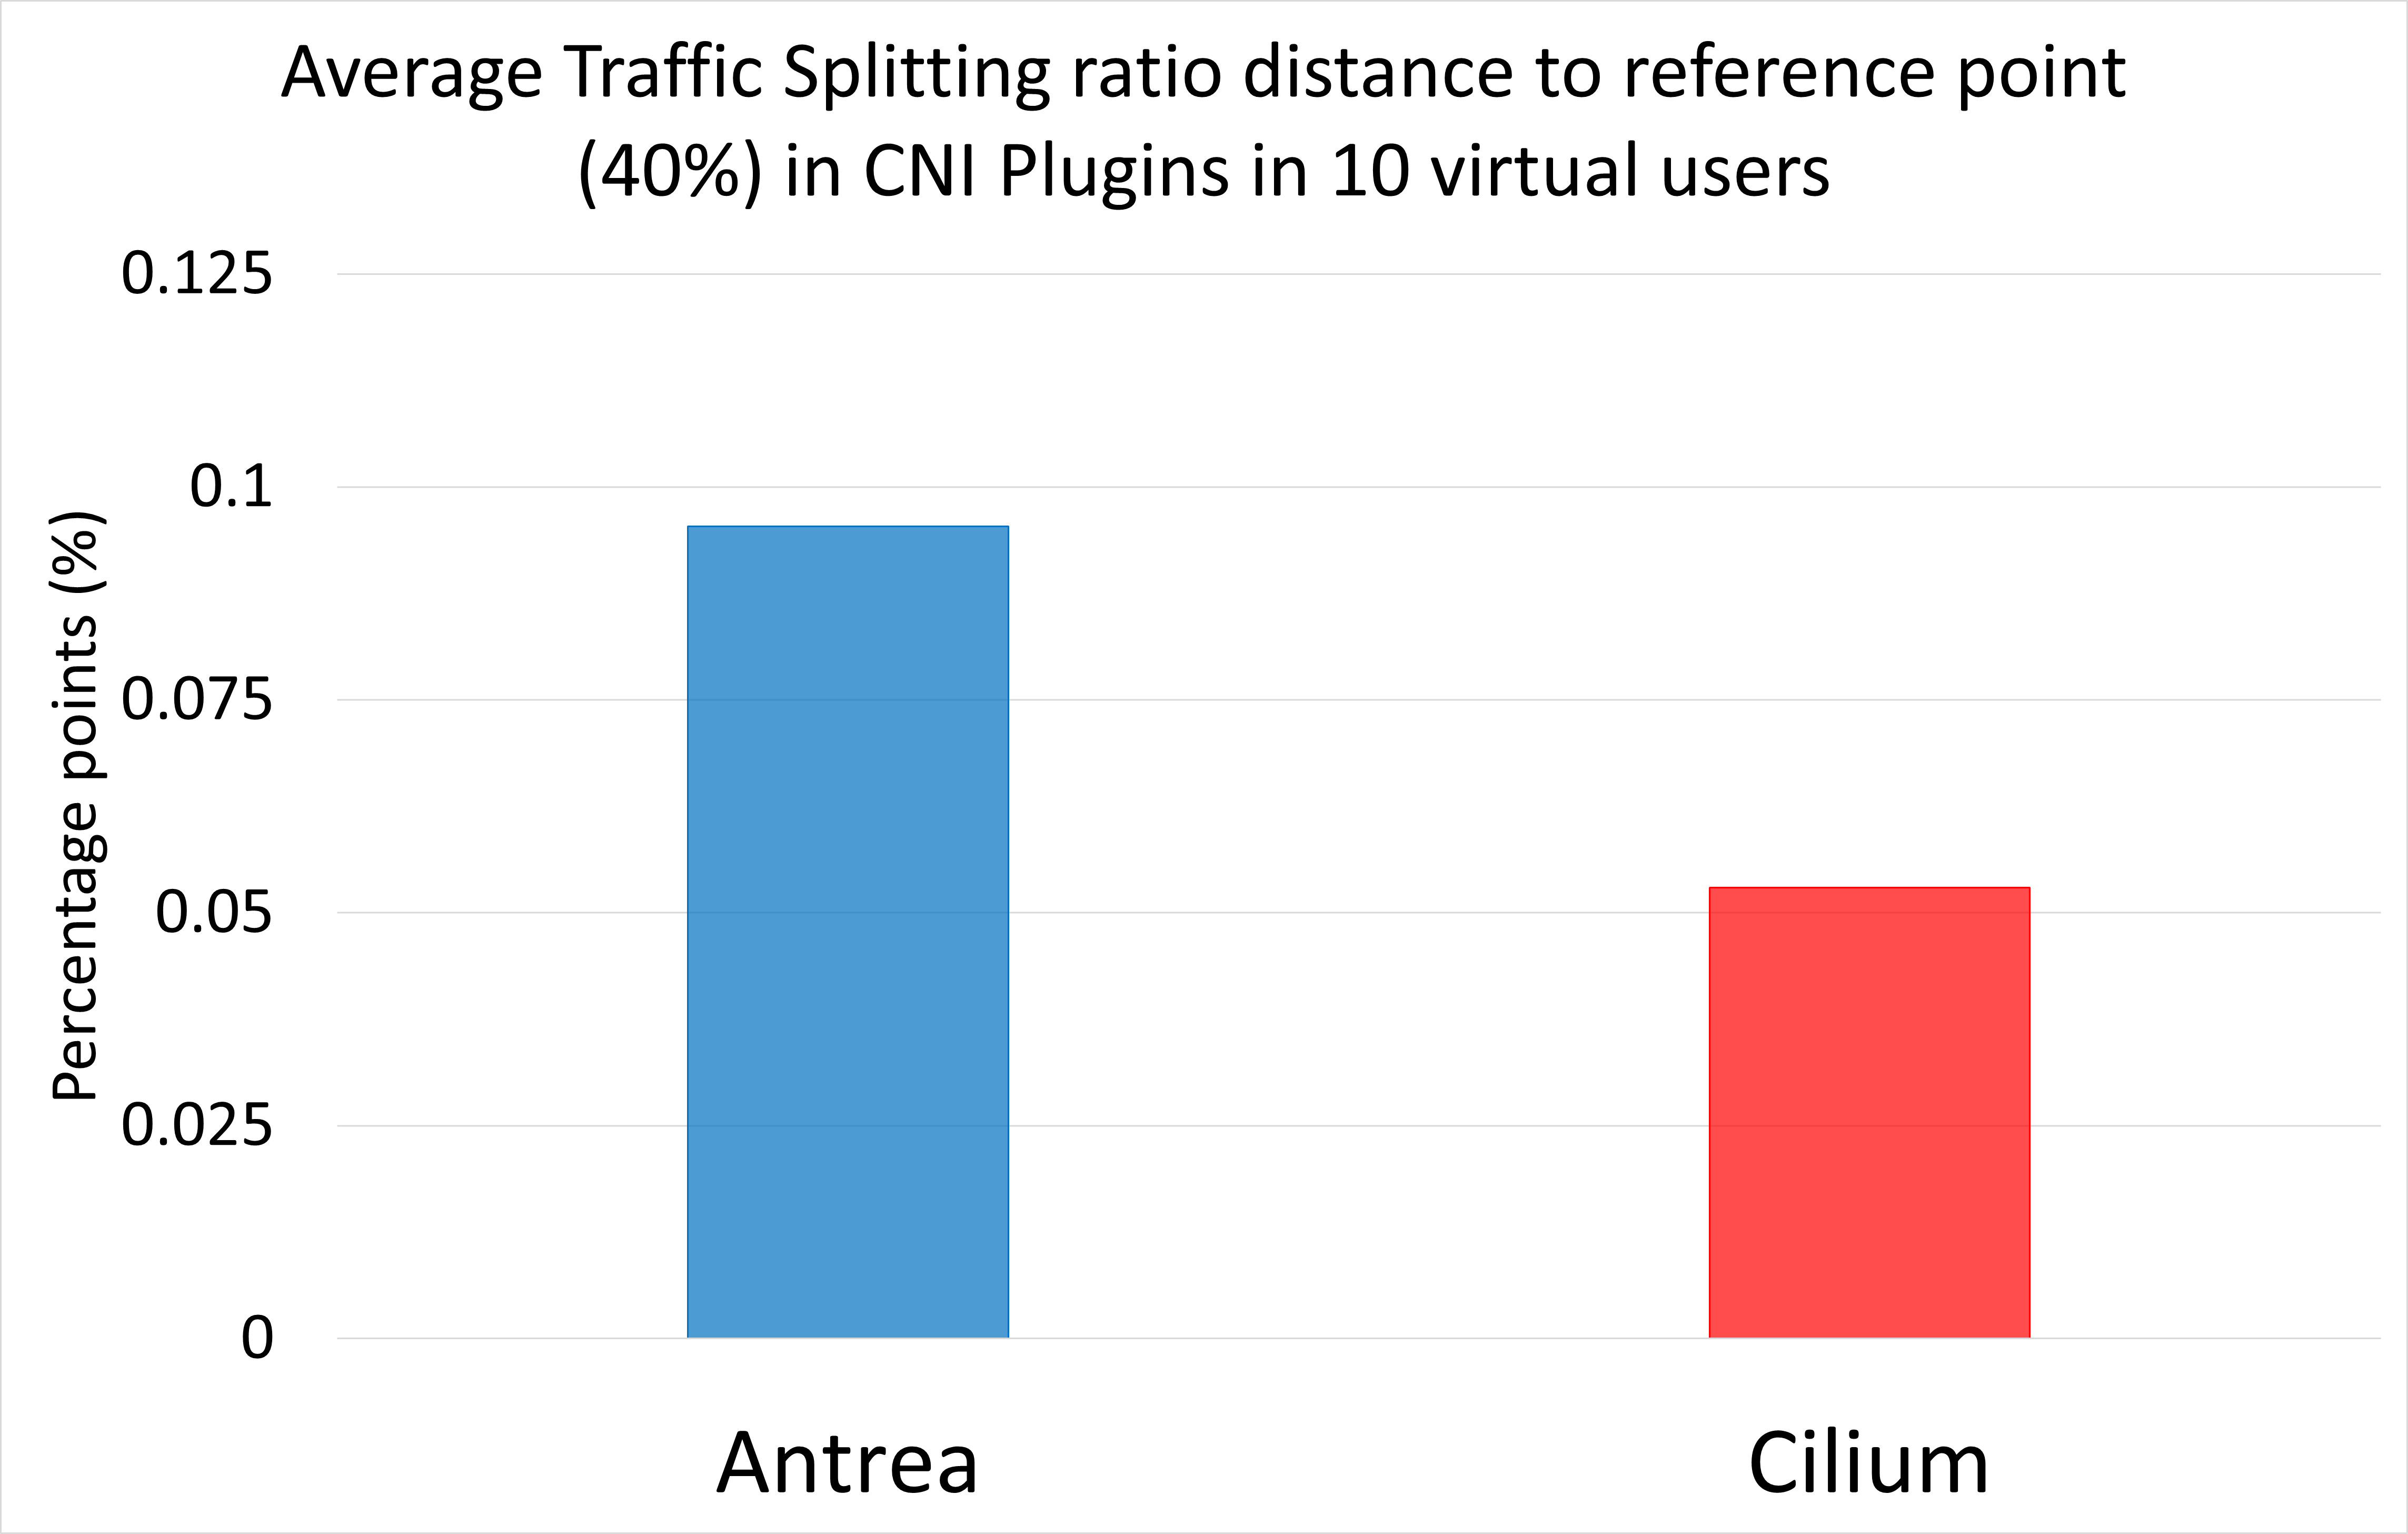
\includegraphics[width=\textwidth]{plots/traffic-splitting/time_window_5_10vu_reference_cloud.png}
        \label{fig:reference_10vu}
        \caption{}
    \end{subfigure}

    \vspace{0.5cm}

    \begin{subfigure}[b]{0.49\textwidth}
        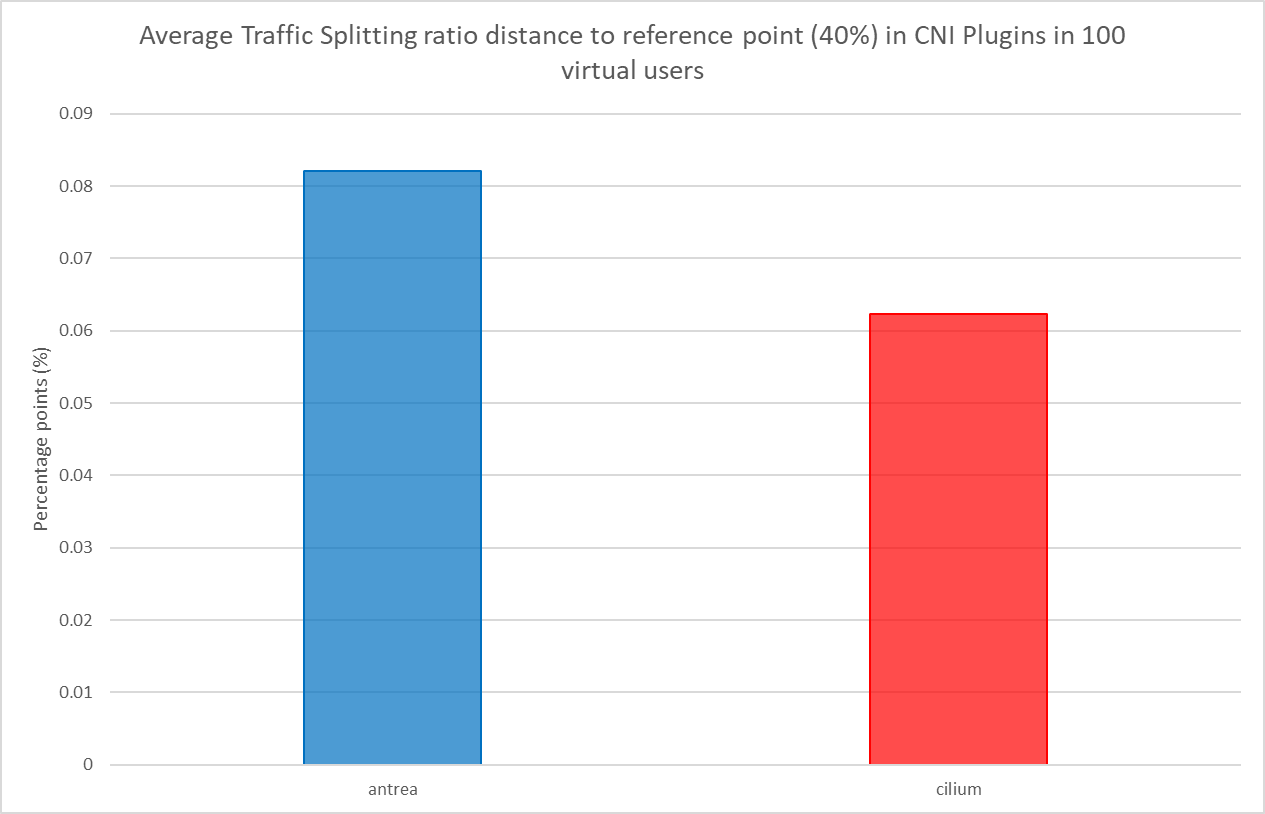
\includegraphics[width=\textwidth]{plots/traffic-splitting/time_window_5_100vu_reference_cloud.png}
        \label{fig:reference_100vu}
        \caption{}
    \end{subfigure}
    \begin{subfigure}[b]{0.49\textwidth}
        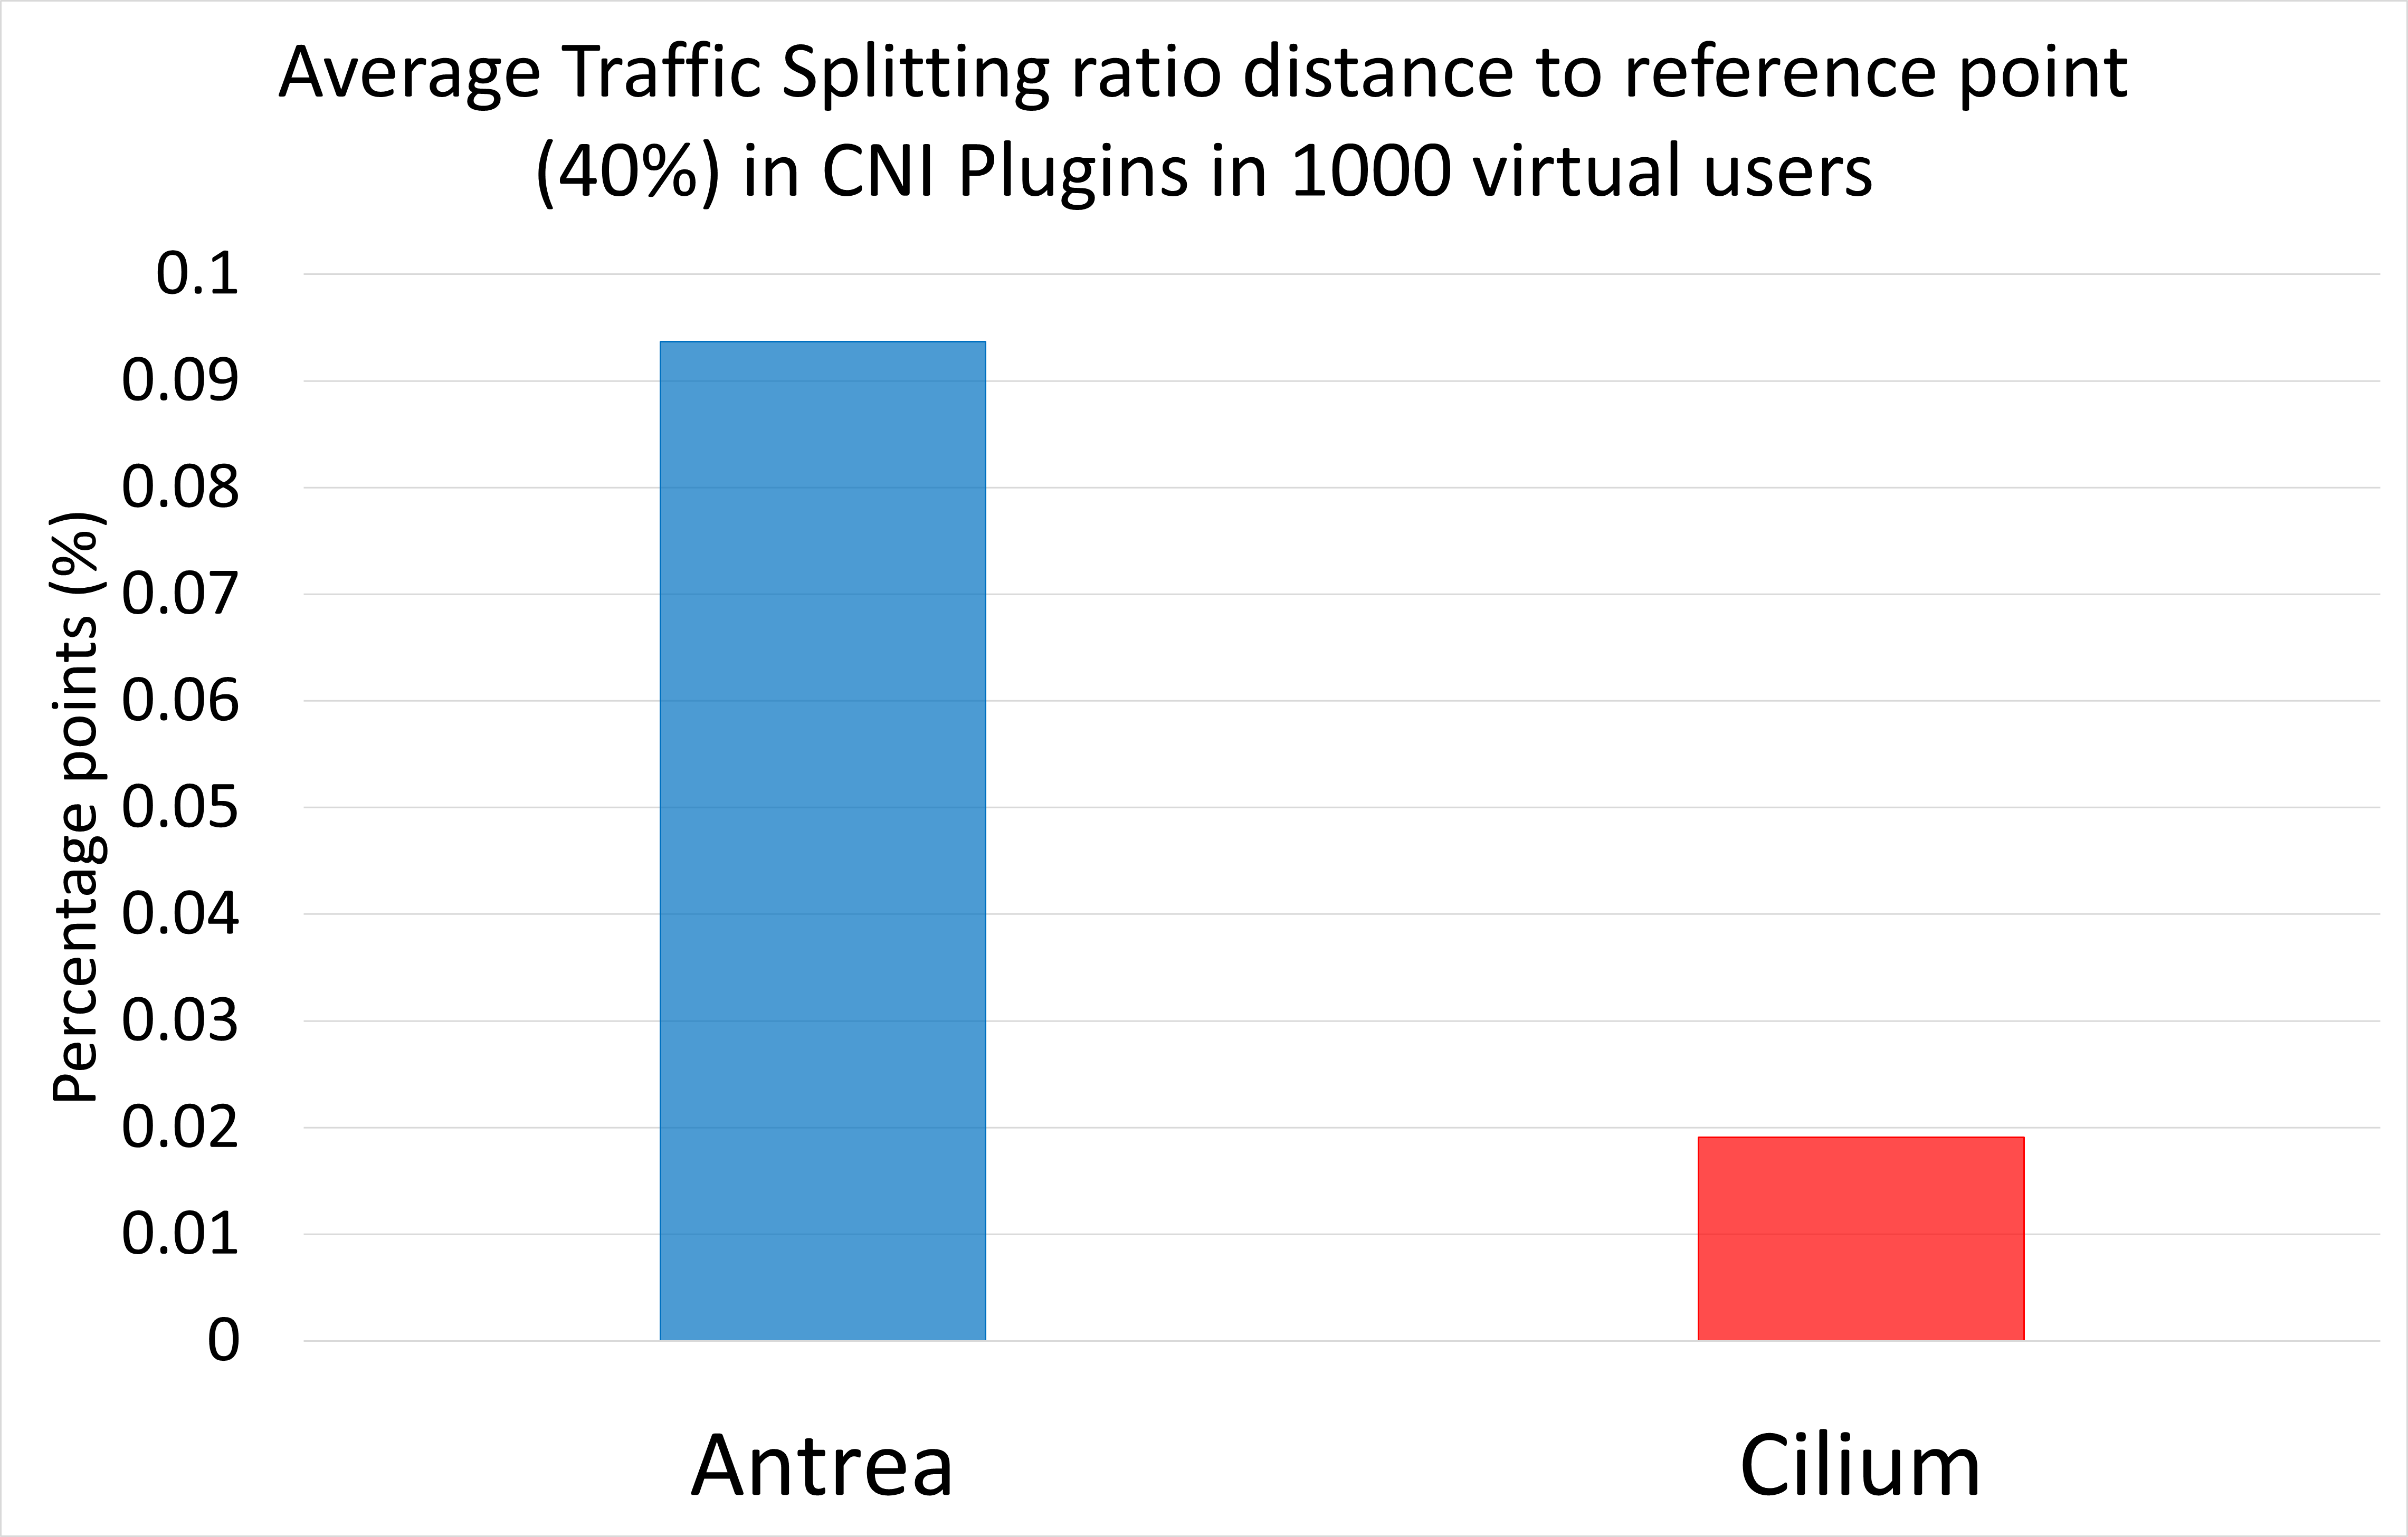
\includegraphics[width=\textwidth]{plots/traffic-splitting/time_window_5_1000vu_reference_cloud.png}
        \label{fig:reference_1000vu}
        \caption{}
    \end{subfigure}

    \caption{Average traffic splitting ratio distance to reference point in increasing virtual users, (a) one, (b) ten, (c) hundred, (d) thousand }
    \label{fig:referencesIngress}
\end{figure}
